\documentclass[a4paper,12pt]{article}
\usepackage{amsmath}
\usepackage{graphicx}
\usepackage{fancyhdr}
\usepackage{placeins}
\usepackage{multirow}
\usepackage{geometry}
\usepackage{subcaption}
\usepackage{float}
\usepackage[bottom]{footmisc}
\geometry{top=20mm, bottom=20mm, left=20mm, right=20mm}
\usepackage{setspace}
\usepackage[style=bath,sorting=ynt]{biblatex}
\usepackage[hyperindex, colorlinks=true, linkcolor=blue, citecolor=blue]{hyperref}
\assignrefcontextentries[]{*}
\addbibresource{references.bib}
\RequireCitationStyle{authoryear-comp}
\ExecuteBibliographyOptions{uniquename=init}
\renewcommand*{\compcitedelim}{\addsemicolon\space}
\raggedbottom

\usepackage{listings}
\usepackage{xcolor}

\definecolor{MatlabBlue}{rgb}{0.0, 0.0, 1.0}        % Blue for keywords
\definecolor{MatlabGreen}{rgb}{0.0, 0.5, 0.0}       % Green for comments
\definecolor{MatlabMagenta}{rgb}{0.75, 0.0, 0.75}   % Magenta for strings
\definecolor{MatlabGray}{rgb}{0.5, 0.5, 0.5}        % Gray for line numbers
\definecolor{MatlabBackground}{rgb}{0.95, 0.95, 0.95} % Light gray background

\lstset{ 
  language=Matlab,                 % Set language to MATLAB
  backgroundcolor=\color{MatlabBackground}, % Background color for the code
  basicstyle=\ttfamily\footnotesize\fontfamily{pcr}\selectfont, % Font style and size (Consolas)
  commentstyle=\color{MatlabGreen},  % Style for comments
  keywordstyle=\color{MatlabBlue},  % Style for keywords
  stringstyle=\color{MatlabMagenta},      % Style for strings
  numbers=left,                     % Line numbers on the left
  numberstyle=\tiny\color{MatlabGray},    % Style for line numbers
  stepnumber=1,                     % Number every line
  numbersep=5pt,                    % Distance between line numbers and code
  showstringspaces=false,           % Don't show spaces in strings
  breaklines=true,                  % Break long lines
  showtabs=false,                   % Don't show tabs
  captionpos=b,                     % Position of the caption (b for bottom)
  escapeinside={\%*}{*)},           % Enable escaping to LaTeX
  frame=single,                     % Add a frame around the code
  rulecolor=\color{black},          % Set color of the frame
  morekeywords={classdef,methods,end,try,catch} % Add MATLAB-specific keywords
}

\begin{document}
\pagestyle{fancy}  
\fancyhf{}  
\doublespacing  

% Adjust header height
\setlength{\headheight}{16pt}       
\addtolength{\topmargin}{-4pt}     


% Header setup
\fancyhead[L]{\fontsize{14}{16}\selectfont  Ultrasonic Sensor-based Object Detection System}  

% Footer setup
\fancyfoot[R]{\thepage}

\begin{titlepage}
  \thispagestyle{empty}
  \centering
  
\includegraphics[width=0.6\textwidth]{figs/uob-logo-grey-transparent-1.png} \\[2cm]
  {\Huge\textbf{Ultrasonic Sensor-based Object Detection System}} \\[1.5cm]
  {\LARGE\textbf{Department of Mechanical Engineering}} \\[0.5cm]
  {\LARGE\textbf{ME12004 S1}} \\[2cm]
  {\Large\textbf{December 27, 2024}} \\[2cm]
  {\Large\textbf{Student Name: Colin Peden}} \\[0.5cm]
  {\Large\textbf{Student Number: CPFP20}} \\[1cm]
  \vfill
\end{titlepage}

\tableofcontents

%TC:ignore
\begin{abstract}
A measurement system combing an Arduino microcontroller and ultrasonic ranging module, controlled via MATLAB script was used to evaluate moving average filtering along with estimating and correcting for measurement errors via calibration against known values. Filtering increased measurement smoothness. Estimated measurement errors were low before calibration, corrections were then made within the control script. The beam angle constraint of the ranging module was evaluated in Task 2 and mitigating methods detailed. For Task 3 a more advanced measurement and alarm system, which could be used as a safety system in a factory, was made. This system included additional inputs such as a light dependent resistor and potentiometer. A more advanced control script, with a graphical user interface, was developed utilising lessons learnt from Task 1.
\end{abstract}
%TC:endignore

\section{Introduction}

\subsection{Task 1: Sensor Circuit and Arduino Setup}

Arduino is an open-source electronics platform with a microcontroller with both digital and analogue inputs and outputs. Ultrasonic ranging modules are sensors which measure distances using ultrasonic pulses.
A test circuit was made using an ultrasonic ranging module and Arduino Uno, controlled via MATLAB script.
It was used to estimate and correct for measurement error through calibration against known distances. It was also used to evaluate and apply moving average filtering. 

\subsection{Task 2: Beam Angle Constraints}
Sensors should be characterised to ensure they are used within their capabilities. Beam angle is a limitation of ultrasonic ranging modules, it affects the region where a sensor can detect a target or accurately measure distance.


\subsection{Task 3: Object Detection and Alarm}

The aim of task 3 was to create a measurement and alarm system controlled by a MATLAB application with a graphical user interface (GUI) that combines measurement and alarm functionality with visual feedback via an LED. This system could be used for safety in a factory by alerting workers to nearing equipment and recording its positions.



\section{Theory}

\subsection{Task 1: Sensor Circuit and Arduino Setup}
Ultrasonic ranging modules utilise the time of flight (TOF) of an ultrasonic pulse emitted and received by the module to estimate the distance of the target which reflected it. TOF can be converted to distance ($D$) using the speed of sound at sea level (343m/s) by this equation:
\begin{equation}
D(m) = \frac{\text{Time of Fight} (s)\times343(m/s)}{2}
\end{equation}

Noise consists of random changes and fluctuations that are not part of a true or wanted signal and arises from many sources including electrical interference and sensor inaccuracies \parencite{Tuzlukov2002}. A moving average filter averages a fixed number of recent data points, the number of data points is referred to as the window size. It is a low-pass filter, reducing higher frequency fluctuations that are more likely to be noise and preserving the likely true signal. Increasing window sizes results in greater smoothing. However, since the average includes older data points it introduces a delay or lag between the filtered signal and any changes in the raw data.
The rolling average equation is given below, where $\text{Rolling Average}(n)$ is the filtered value at data point $n$, $x_i$ are the raw data points and $k$ is the window size:

\begin{equation}
\text{Rolling Average}(n) = \frac{1}{k} \sum_{i=n-k+1}^{n} x_i
\end{equation}


Measurement error, the difference between the true value and the observed value, can be reduced by calibration. This requires comparing observed measurements to known values and then applying a correction to fit the measured data to the known values.


\subsection{Task 2: Beam Angle Constraints}
Ultrasonic sensors work by sending a directional pulse that is reflected back, as such there is a limit to the angle an object can be from the sensor to still be measured. As the pulses travel, they spread, dispersing their energy. Pulses with smaller beam angles can travel further before being dissipated. Additionally, as the HC-SR504 sensor sends groups of 8 pulses (Appendix~\ref{trusens}), it is possible that some of the transmitted pulses could interfere with reflected pulses, affecting the accuracy of the sensor at different angles. 
The perpendicular distance ($h$) from the centre line of the sensor at a given distance in front ($D_{I}$) can be converted to an angle ($\theta$) using the equation: 
\begin{equation}
\theta = \arctan\left( \frac{h}{D_{I}} \right)
\end{equation}

Additionally at a given $D_{I}$, the expected distance ($D_{E}$) increases as $h$ does. This can be calculated using the length of the hypotenuse of a triangle:
\begin{equation}
D_{E} = \sqrt{D_{I}^2+h^2}
\label{eq:4}
\end{equation}


\subsection{Task 3: Object Detection and Alarm}
Below is an equation defining the flashing frequency ($f$) of an alarm based on the output voltage of a potentiometer ($V_{Out}$) and a distance ($D$):

\begin{equation}
\label{alarm}
    f = 10 \times V_{Out} \times \frac{1}{D}
\end{equation}

A light dependant resistor (LDR) ($R_1$) can be used in a potential divider with another resistor ($R_2$) to provide an output voltage ($V_{Out}$) that increases with the amount of light incident on the sensor:

\begin{equation}
\label{ldr}
V_{Out} = V_{In} \times \frac{R_2}{R_1 + R_2}
\end{equation}

MATLAB programs typically run on a single logical processor meaning the program runs sequentially and any function must wait for the prior. One solution is a parallel worker that runs a function outside the main program.





\section{Methodology}
\subsection{Task 1: Sensor Circuit and Arduino Setup}
Figure~\ref{fig:circuit_diagram} details how the sensor was connected to an Arduino Uno microcontroller with 5v, ground, trigger (yellow) and echo (orange) pins.

\begin{figure}[htbp]
    \captionsetup{justification=centering}
    \centering
    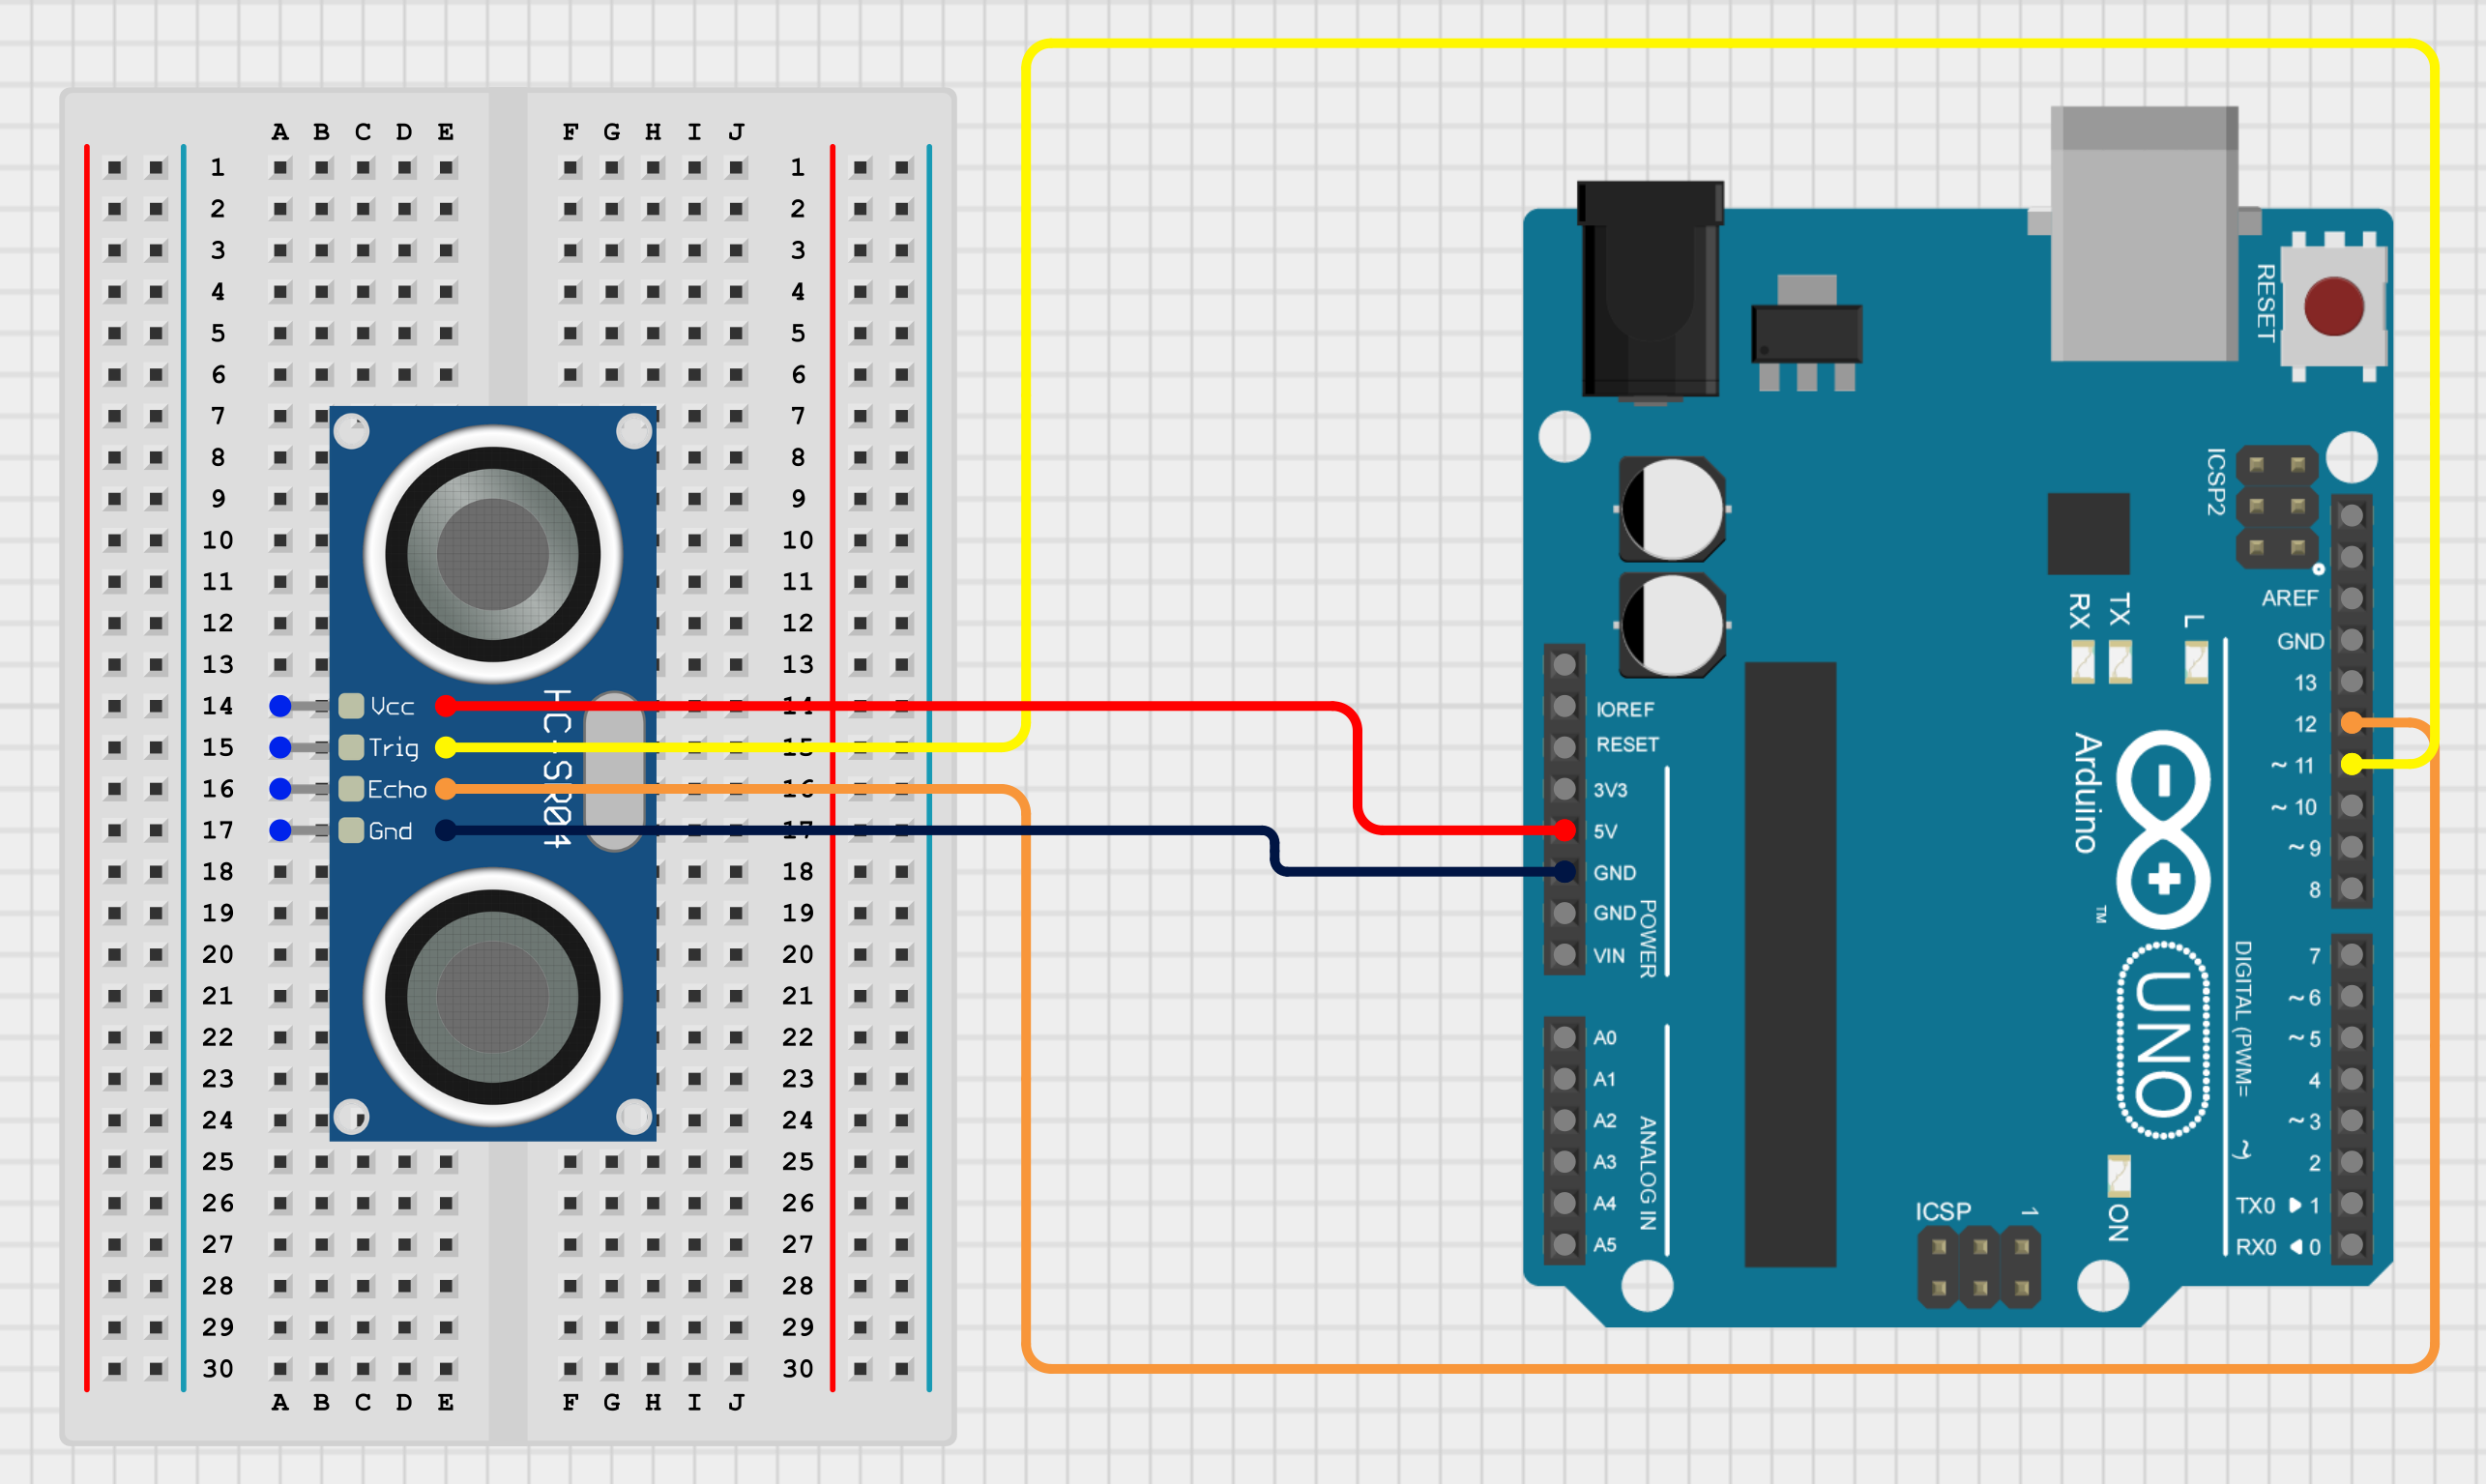
\includegraphics[width=0.8\textwidth]{figs/task1_circuit.png}
    \caption{Circuit diagram of Task 1.}
    \label{fig:circuit_diagram}
\end{figure}

A MATLAB script utilising the support package for Arduino hardware, which sets up serial communication, was used to control the measurement system (Appendix~\ref{appendix:A1}).

During calibration and initial testing the maximum reliable measurement frequency was 24 Hz and a duration of 10 seconds was used.
All measured distances were set with a tape measure ($\pm$1mm).
Moving average filter window sizes were compared using a measurement of a known distance of 1m (Appendix~\ref{rollingAvgPlots.m}).
For calibration, filtering was applied with a 25 point window size. Measurements from 0.1m to 2m were taken in 0.1m increments (Appendix~\ref{appendix:A2}). A linear model was fitted and a gradient correction and offset calculated, then applied (Appendix~\ref{appendix:A1}).
The experimental setup is shown in Figure~\ref{fig:setup}.

\begin{figure}[htbp]
    \centering
    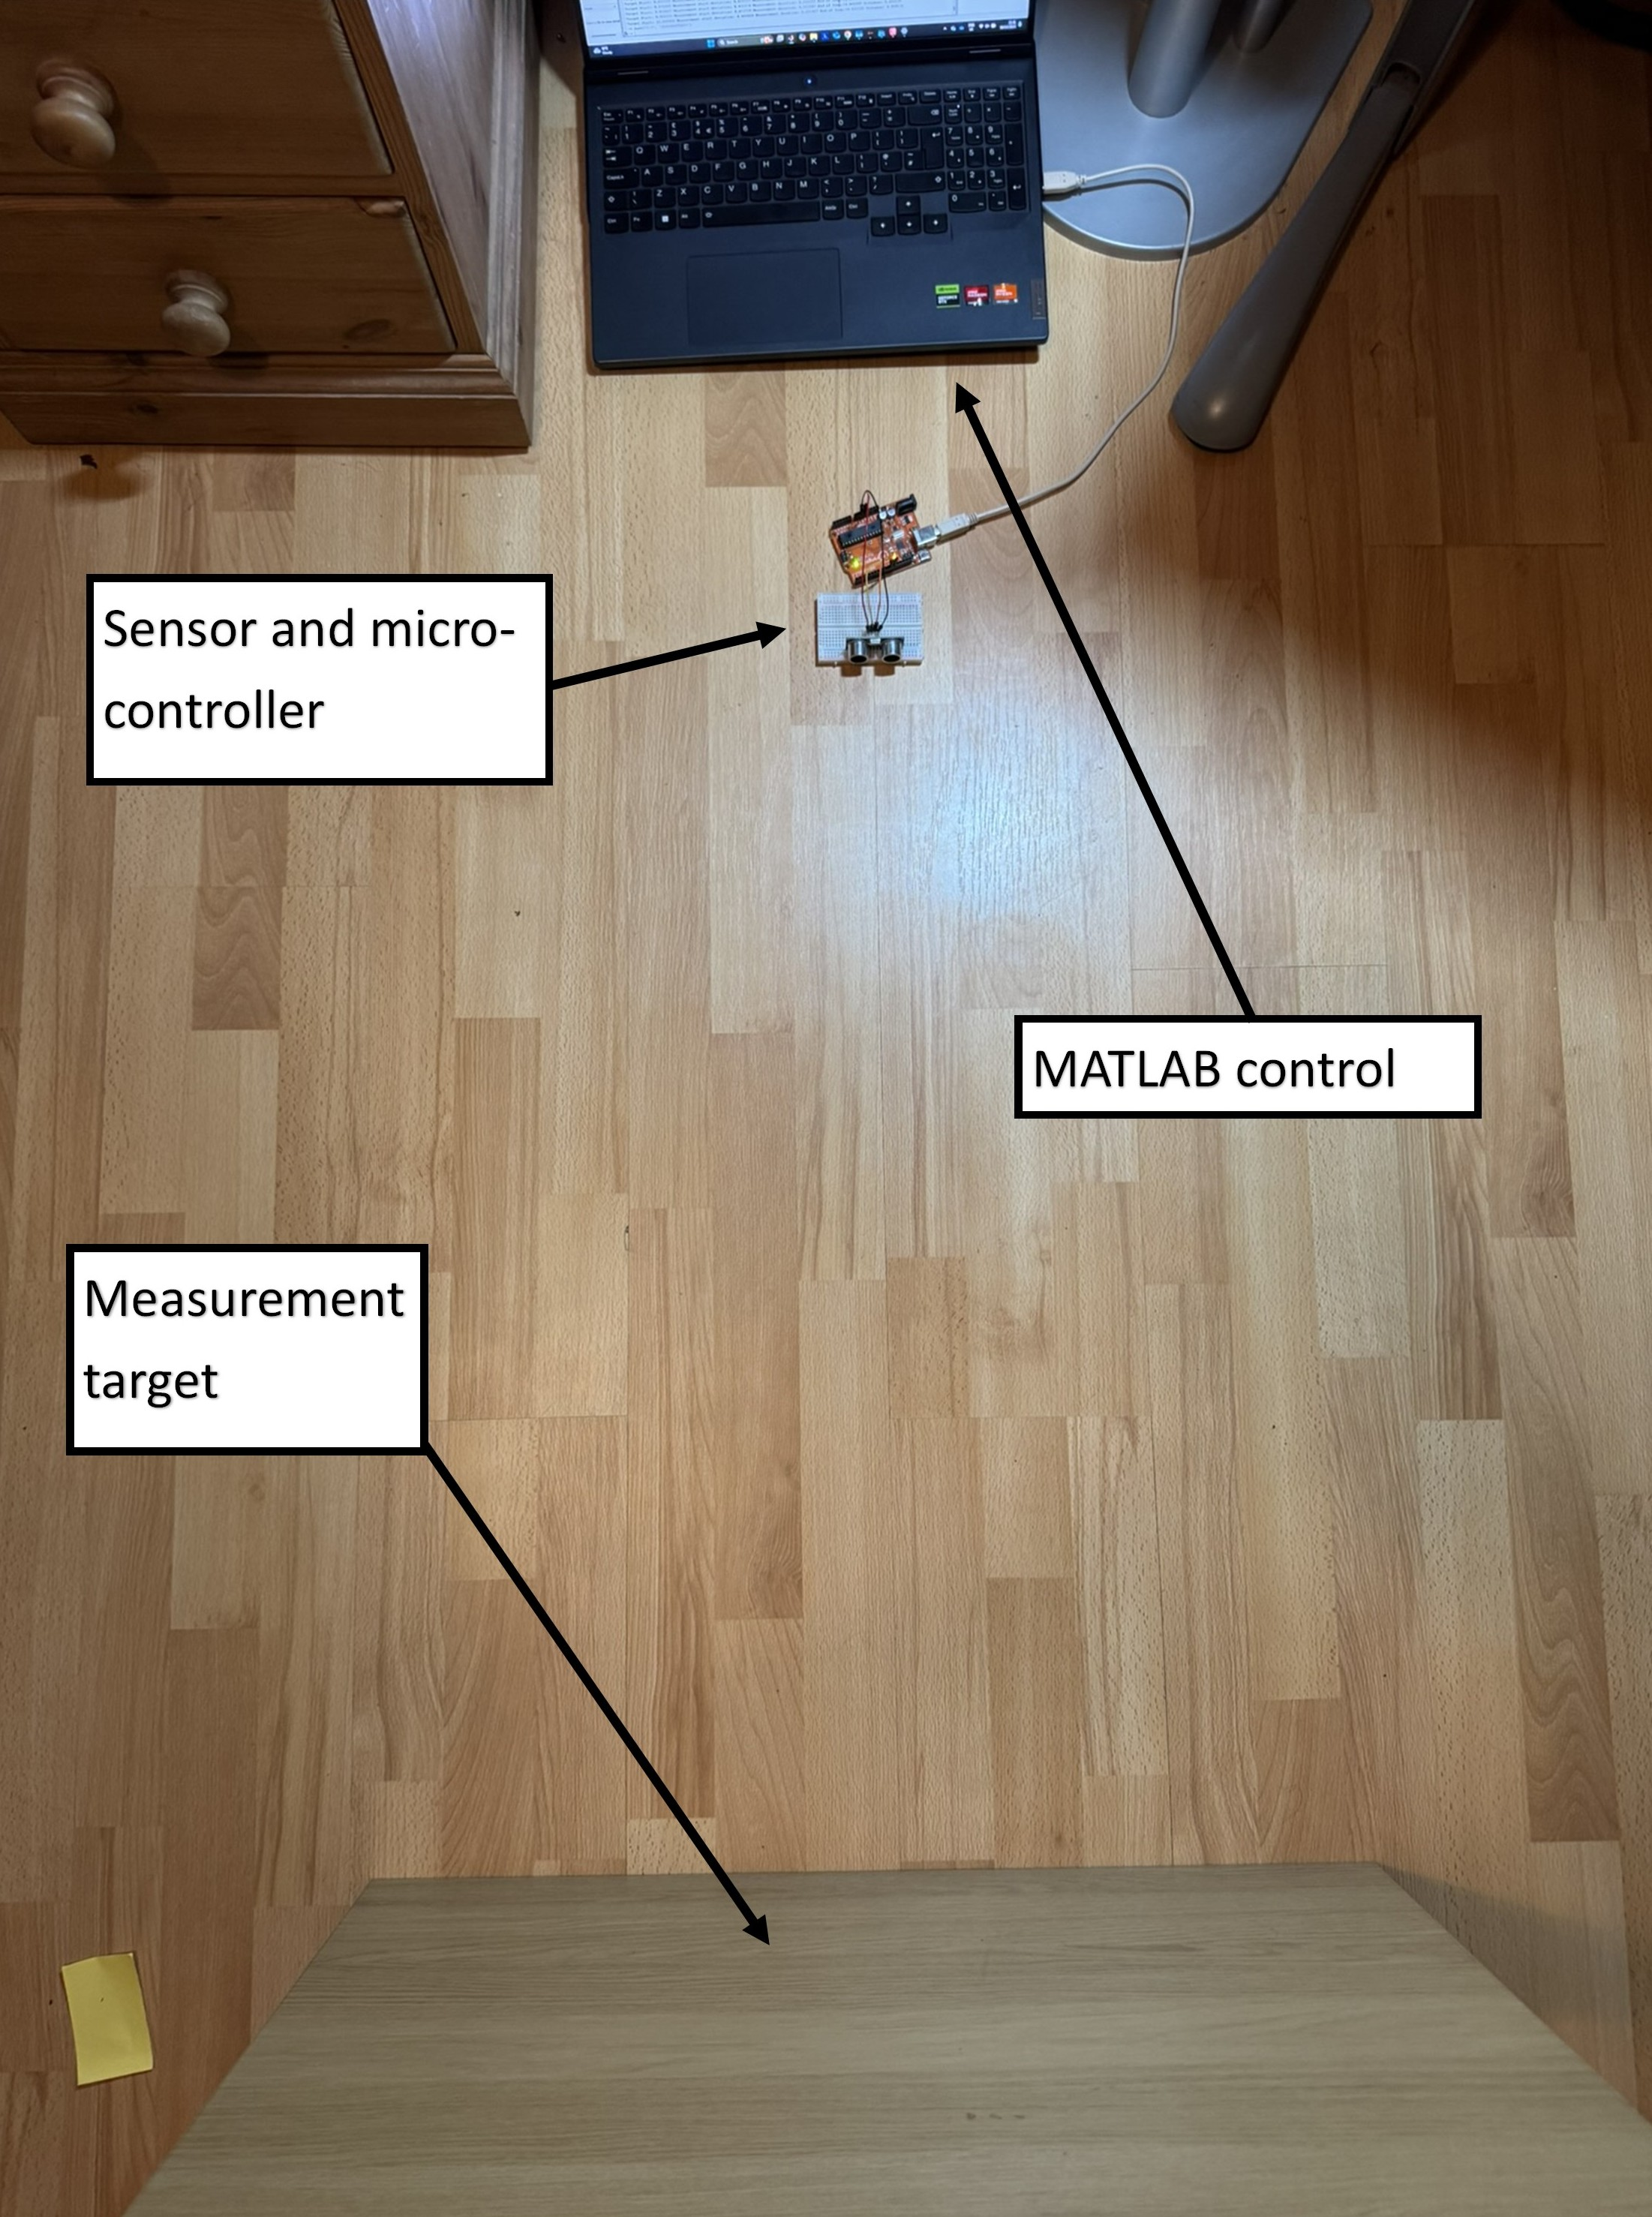
\includegraphics[width=0.45\textwidth]{figs/page01.jpg}
    \caption{Experimental setup for calibration.}
    \label{fig:setup}
\end{figure}

\break

\subsection{Task 2: Beam Angle Constraints}
The measurement system from task 1 was reused. Measurements were taken of a target 0.5m away, moving its edge 1cm at a time from the centre line in either direction. The target was orientated so its body was beyond the edge position. A measurement frequency of 24Hz and duration of 10 seconds was used. 
The experimental setup is shown in Figure~\ref{fig:setup2}.

\begin{figure}[htbp]
    \centering
    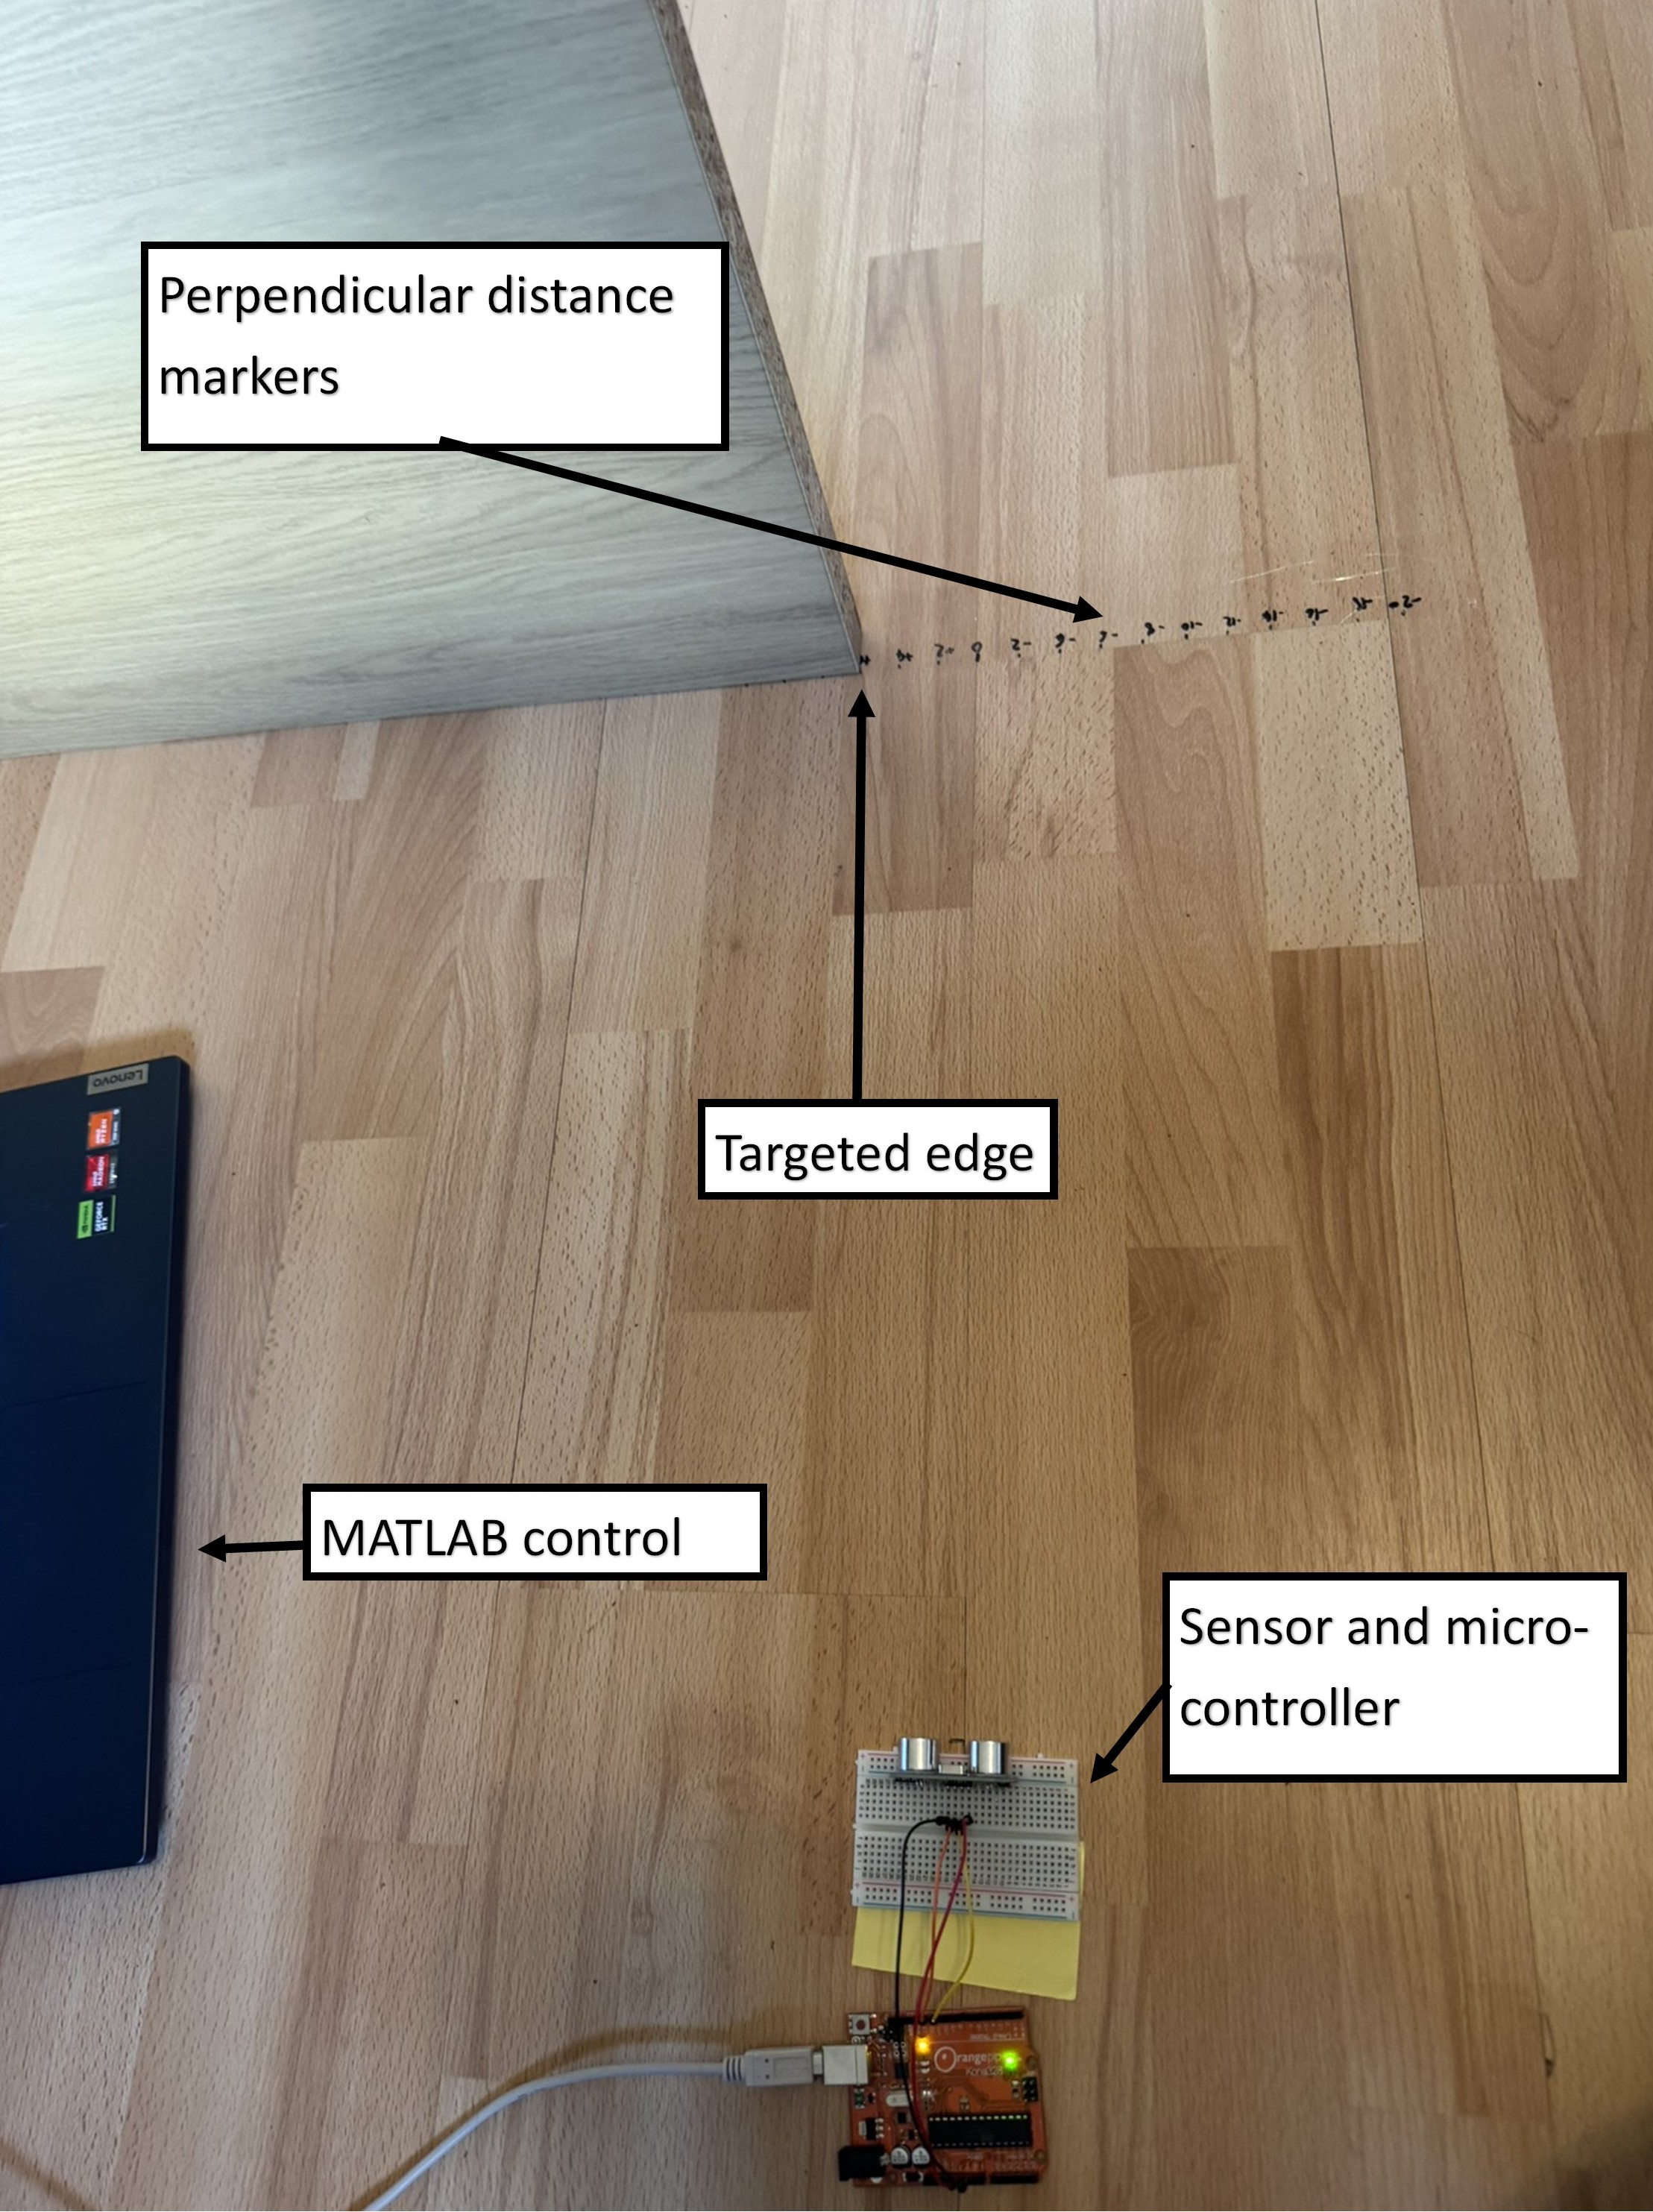
\includegraphics[width=0.45\textwidth]{figs/page02.jpg}
    \caption{Experimental setup for task 2.}
    \label{fig:setup2}
\end{figure}

\break

\subsection{Task 3: Object Detection and Alarm}
The system was made with an Arduino Uno, ultrasonic ranging module, potentiometer, LDR, push-button switch and LED, a schematic is shown in Figure~\ref{fig:task3circuitSchem} and a picture in Figure~\ref{fig:task3circuitPic}.

\begin{figure}[htbp]
    \centering
    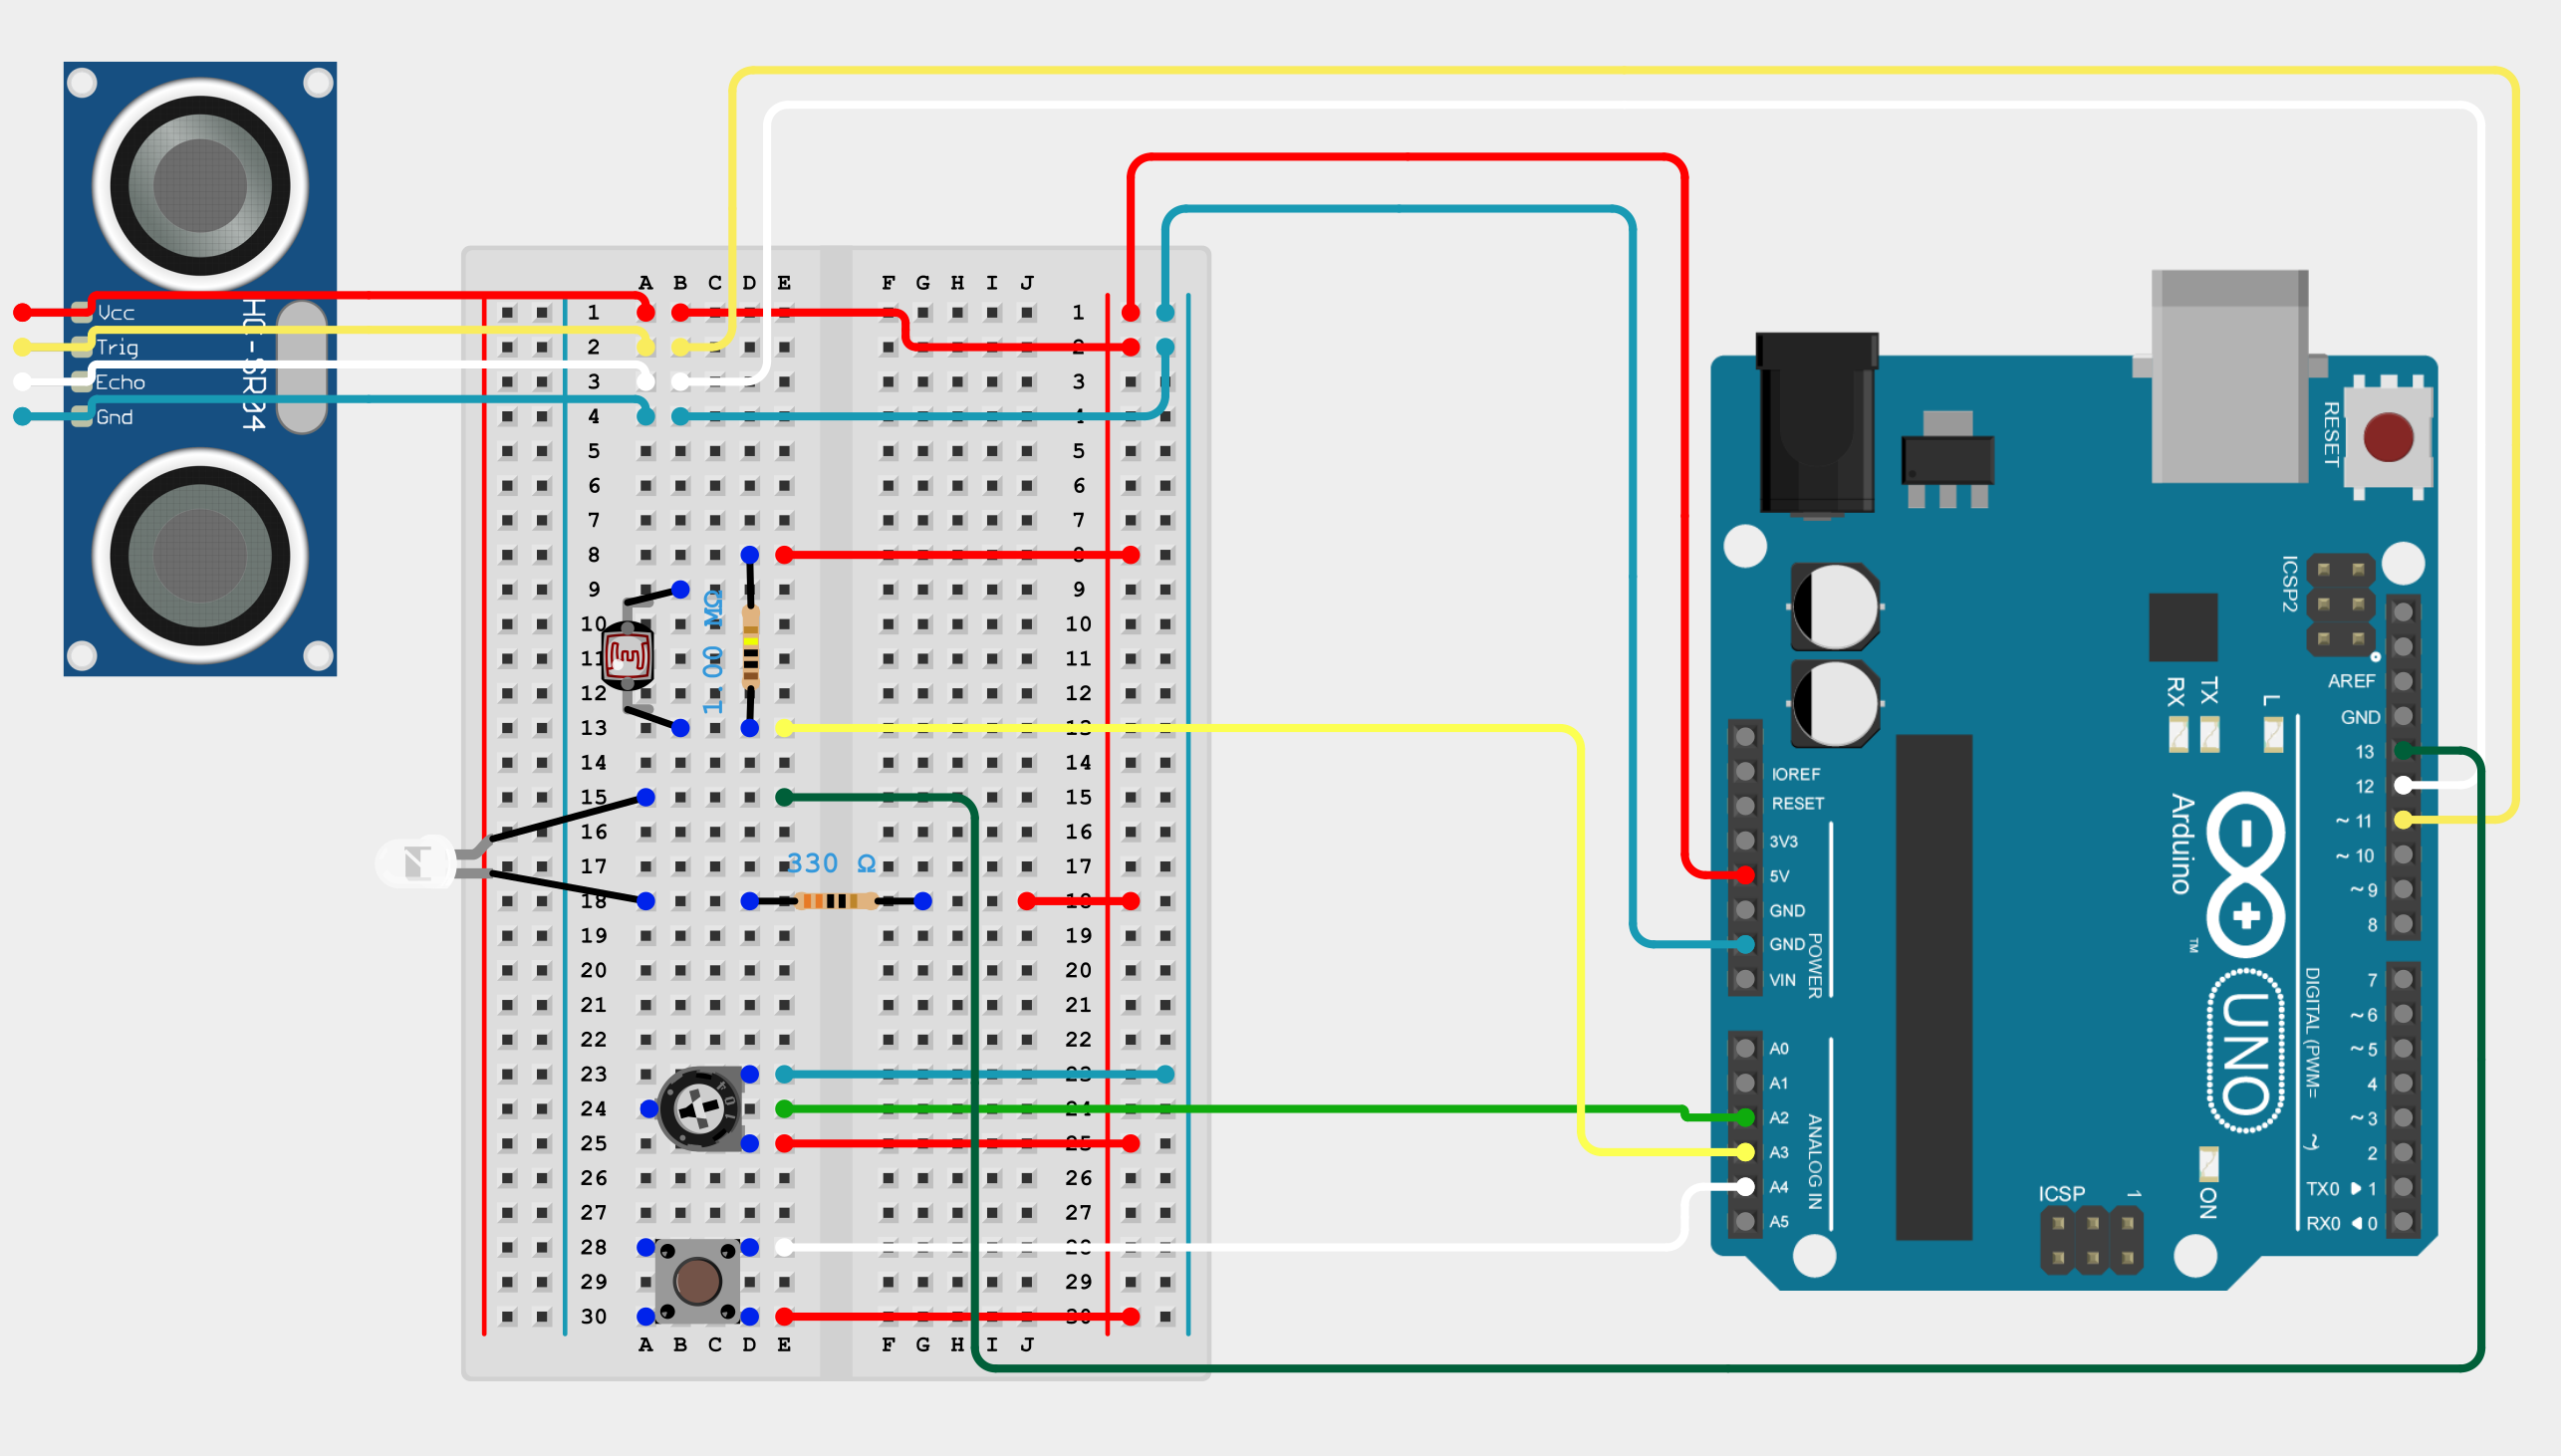
\includegraphics[width=0.8\textwidth]{figs/task3Circuit.png}
    \caption{Circuit Schematic for measurement and alarm system.}
    \label{fig:task3circuitSchem}
\end{figure}

\begin{figure}[htbp]
    \centering
    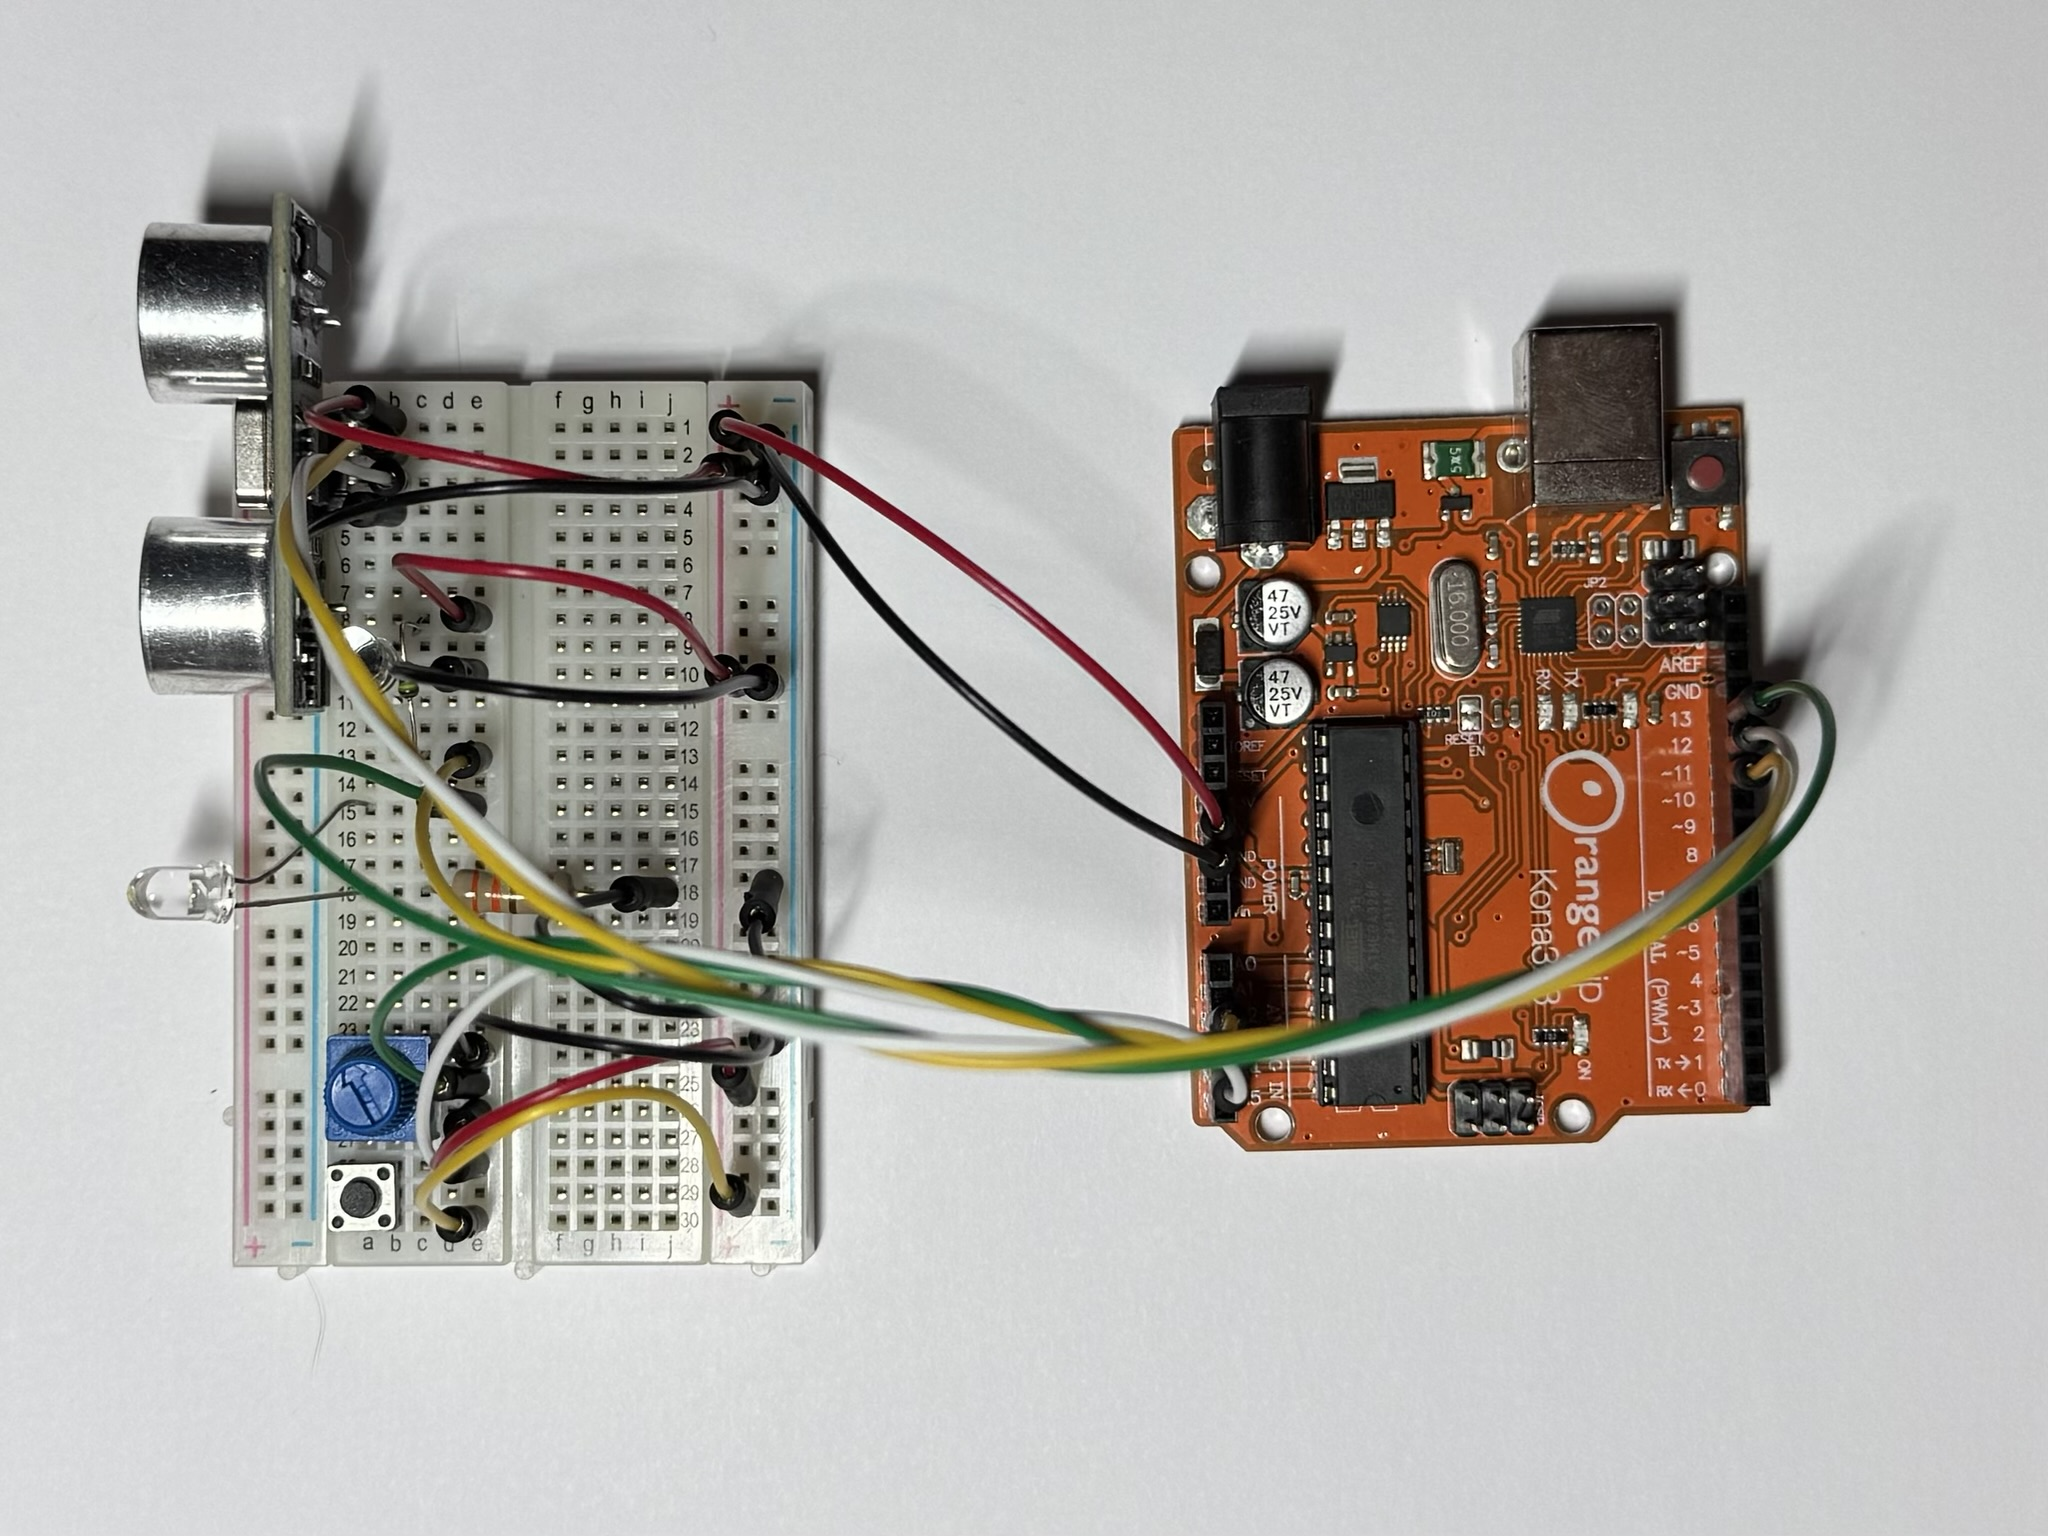
\includegraphics[width=0.8\textwidth]{figs/IMG_3416.JPEG}
    \caption{Circuit for measurement and alarm system.}
    \label{fig:task3circuitPic}
\end{figure}

The GUI outline was created with the MATLAB app designer, all other development was done manually. The application inputs frequency, window size and alarm threshold then plots live distances and displays rolling average and frequency. A toggle enables the alarm (Equation~\ref{alarm}) and another requires the LDR to register low light (Equation~\ref{ldr}) for the alarm to flash. The push-button can record measurements when another toggle is switched. Data is calibrated and filtered as in task 1. The application can also record measurements with timestamps and write them to a .CSV file. A parallel worker using non-blocking logic and a data-queue to output data was used (Appendix~\ref{Appendix:C} Lines:204-320). Data is handled in a circular buffer. Measurements outside calibration range of 0.1-2m are displayed in red.



\break

\section{Results}

\subsection{Task 1: Sensor Circuit and Arduino Setup}
A baseline 1m measurement without filtering or calibration is shown in Figure~\ref{fig:1mBefore}, also a comparison between different moving average window sizes is shown in Figure~\ref{fig:4windowsize}. Averages and standard deviations ($\sigma$) are detailed in Table~\ref{tab:4mean_sd}. The baseline measurement was replotted with the chosen 25 point window moving average filter in  Figure~\ref{fig:1mAfter}.

\begin{figure}[htbp]
    \centering
    \begin{subfigure}[b]{0.45\textwidth}
        \centering
        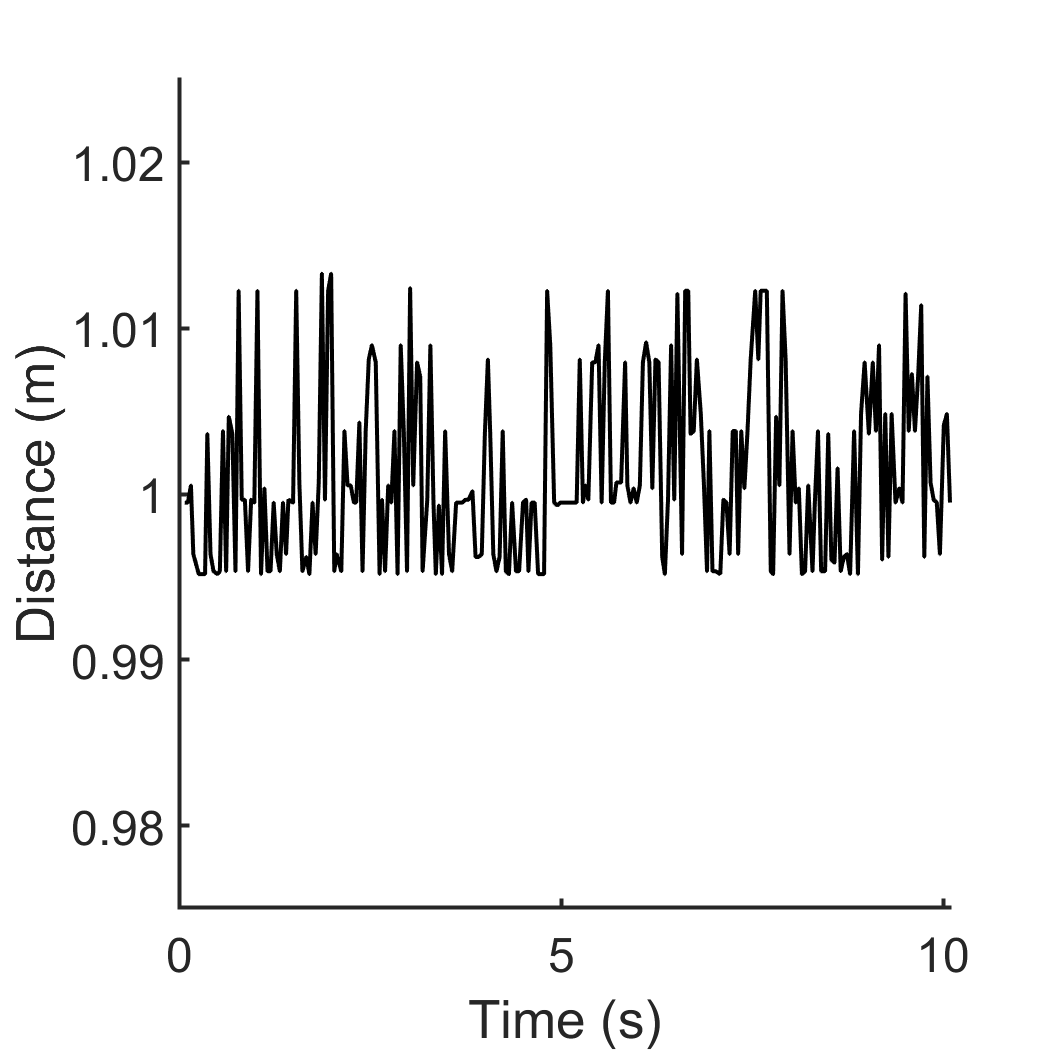
\includegraphics[width=\linewidth]{figs/noRollingAvg.png}
        \caption{Baseline measurement of an object at 1m distance with no filtering or calibration.}
        \label{fig:1mBefore}
    \end{subfigure}\hfill
    \begin{subfigure}[b]{0.45\textwidth}
        \centering
        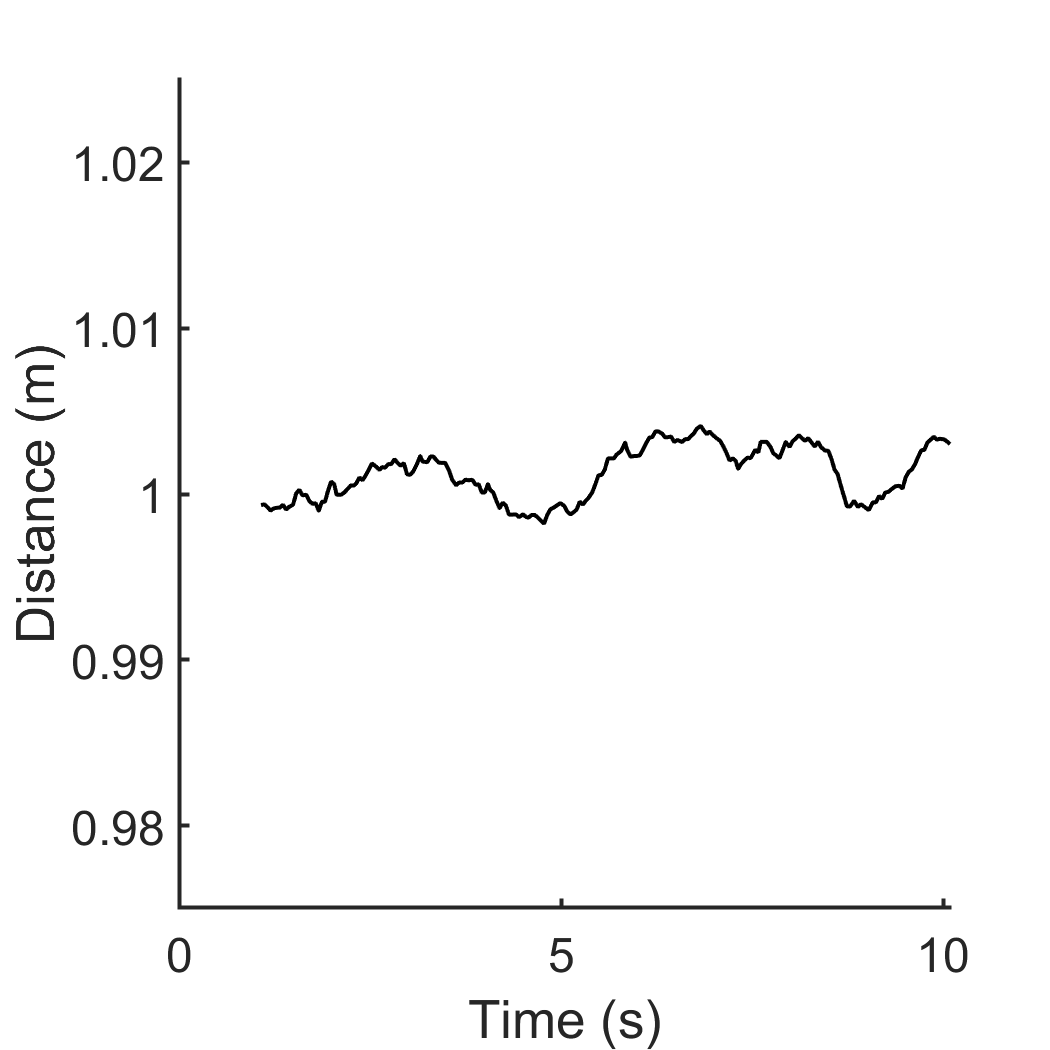
\includegraphics[width=\linewidth]{figs/withRollingAvg.png}
        \caption{Baseline measurement of an object at 1m distance with filtering and no calibration.}
        \label{fig:1mAfter}
    \end{subfigure}
    \caption{Baseline measurement at 1m distance with and without filtering, no calibration}
    \label{fig:1mComparison}
\end{figure}

\begin{figure}[htbp]
    \centering
    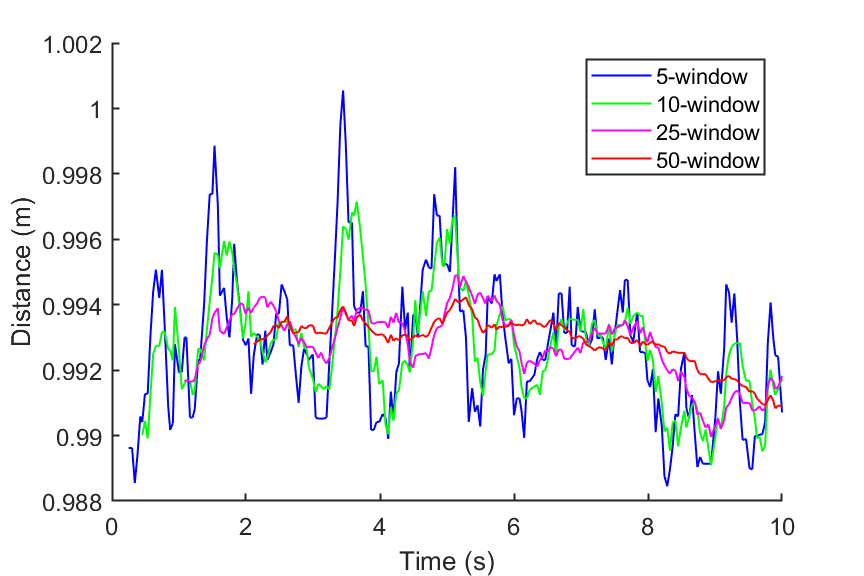
\includegraphics[width=0.8\textwidth]{figs/4windowSizes.png}
    \caption{Measurement of an object at 1m distance with a range of rolling average window sizes and no calibration.}
    \label{fig:4windowsize}
\end{figure}

\begin{table}[htbp]
    \centering
    \caption{Mean and Standard Deviation ($\sigma$) for Different Window Sizes}
    \label{tab:4mean_sd}
    \begin{tabular}{lcc}
        \hline
        \textbf{Window Size} & \textbf{Mean (m)} & \textbf{$\sigma$ (m)} \\
        \hline
        Window 5  & 0.993 & 0.00216  \\
        Window 10 & 0.993 & 0.00168  \\
        Window 25 & 0.993 & 0.00108  \\
        Window 50 & 0.993 & 0.000759 \\
        \hline
    \end{tabular}
\end{table}

Figure~\ref{fig:allcalibration} shows continuous data from each distance used during the calibration process. Figure~\ref{fig:calibration} shows the mean distances, ideal line and fitted linear model, with the model's coefficients shown in Table~\ref{tab:linearModel}. 

\begin{table}[ht]
    \centering
    \begin{tabular}{lcc}
        \hline
        \textbf{Variable} & \textbf{Coefficient} & \textbf{SE} \\
        \hline
        Intercept(mm) & -1.35 & 1.96 \\
        Gradient & 0.998 & 0.00163 \\
        \hline
    \end{tabular}
    \caption{Linear Model Coefficients and Standard Errors.}
    \label{tab:linearModel}
\end{table}

\begin{figure}[htbp]
    \centering
    \begin{minipage}{0.45\textwidth}
        \centering
        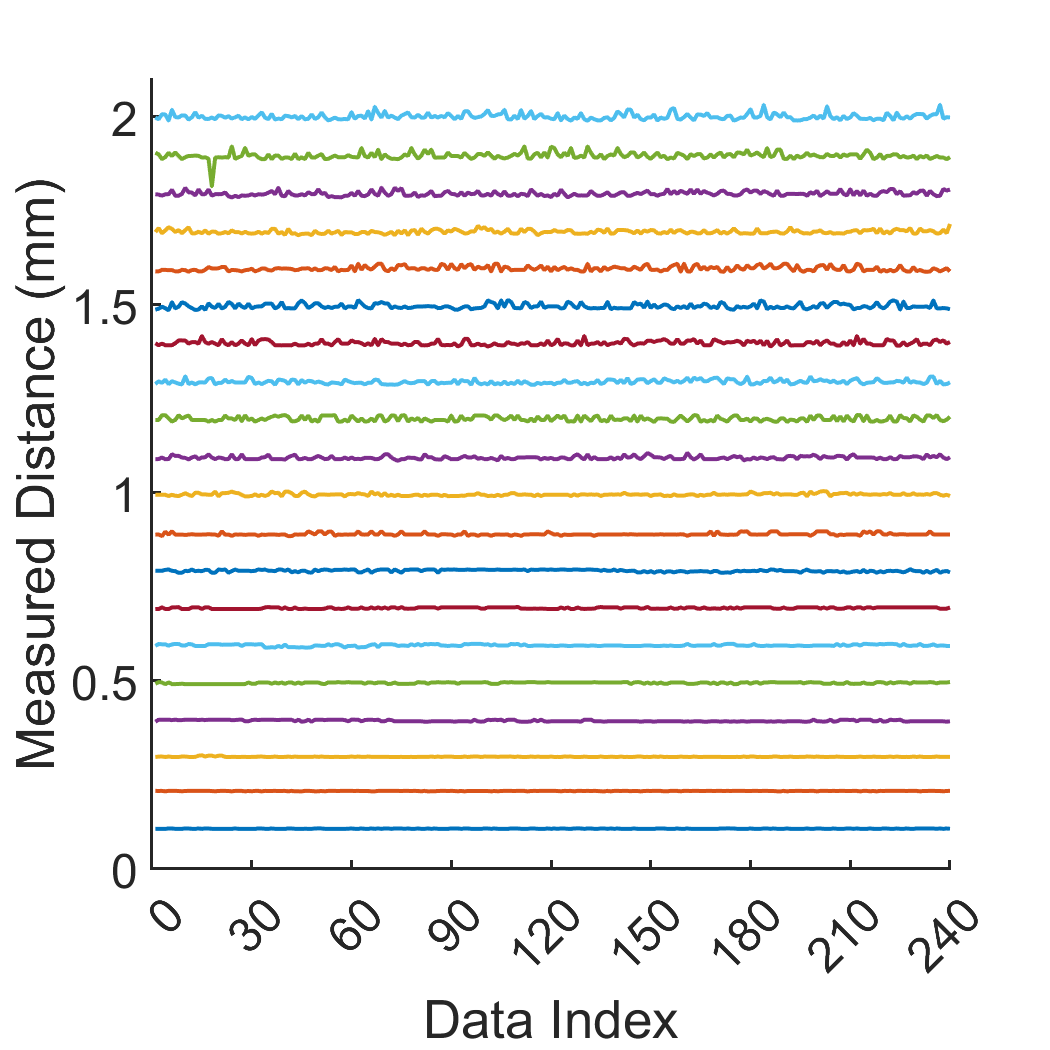
\includegraphics[width=\linewidth]{figs/allCallibration.png}
        \caption{A plot of measurement data used for sensor calibration.}
        \label{fig:allcalibration}
    \end{minipage}\hfill
    \begin{minipage}{0.45\textwidth}
        \centering
        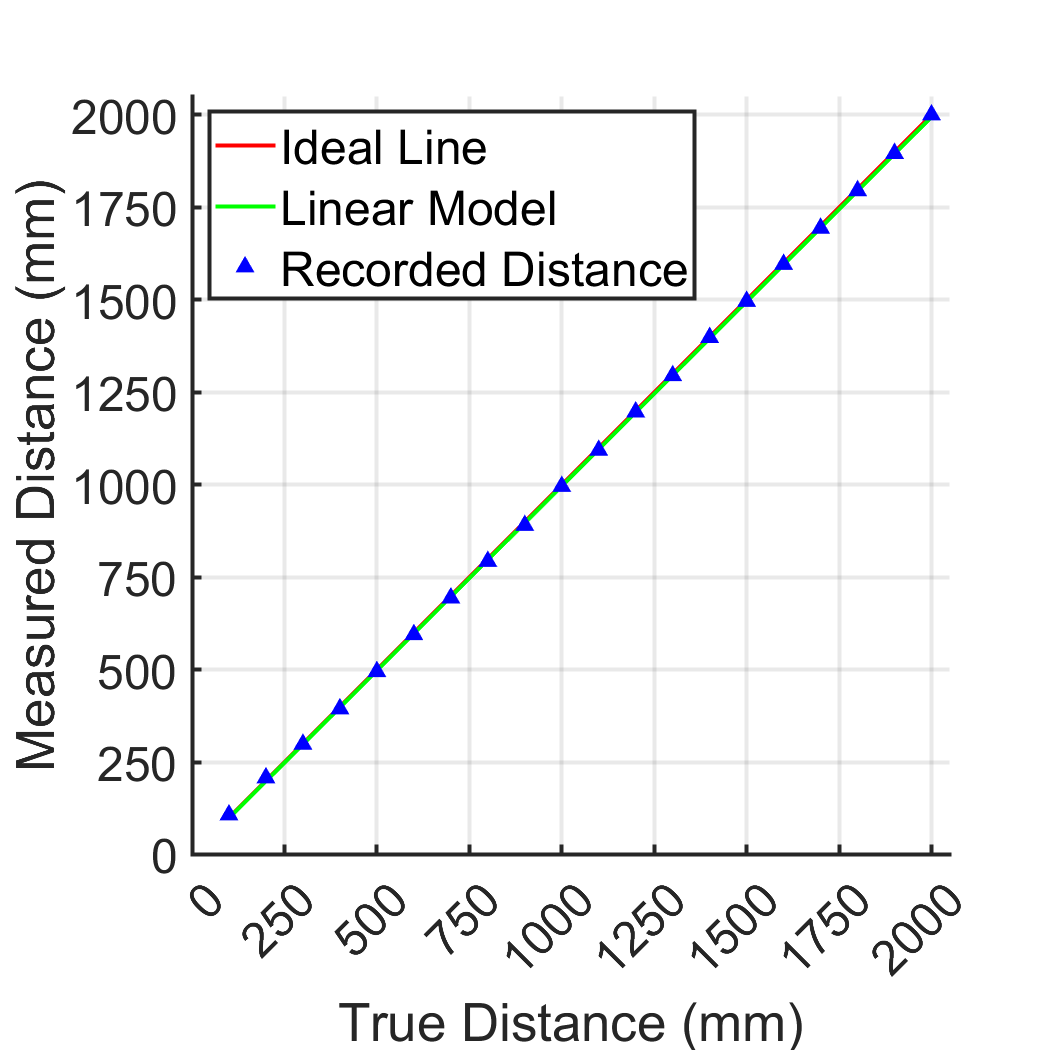
\includegraphics[width=\linewidth]{figs/calibration.png}
        \caption{The average measured distances, linear model, and ideal line for calibration data.}
        \label{fig:calibration}
    \end{minipage}
\end{figure}



To demonstrate live measuring of distance with a moving average after calibration, measurements were taken at a distance of 1m to 0.5m, see Figure~\ref{fig:liveData}

\begin{figure}[htbp]
    \centering
    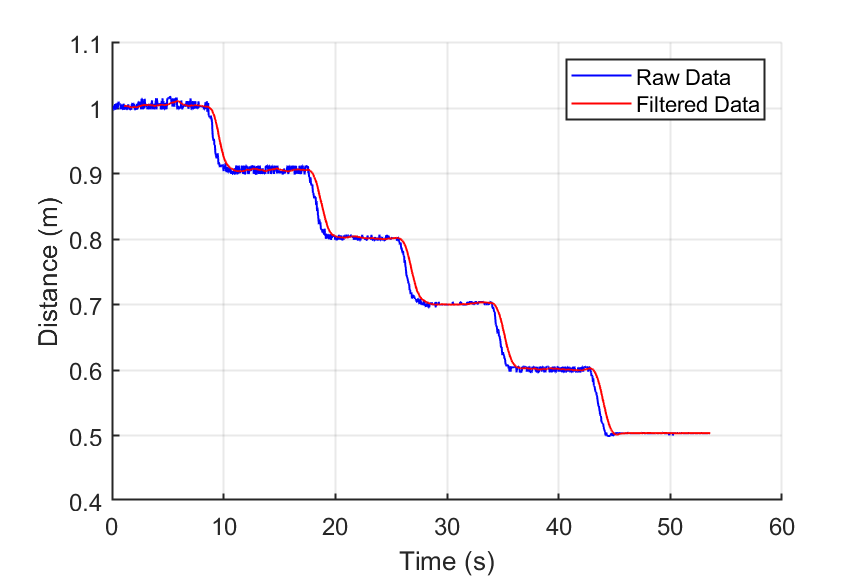
\includegraphics[width=0.8\textwidth]{figs/liveData.png}
    \caption{Measurements of a target's distance at 0.1m increments.}
    \label{fig:liveData}
\end{figure}

\break


\subsection{Task 2: Beam Angle Constraints}
Figure~\ref{fig:distandSE} plots the average distance measured ($D_M$) and $\sigma$ for each $h$.
Average $D_{M}$ is plotted with $D_{E}$ for each $h$ in Figure~\ref{fig:distandExpected}.
The perpendicular distances ($h$) at $D_{I}=0.5$m are converted to angles ($\theta$) in Table~\ref{tab:angles}


\begin{figure}[htbp]
    \centering
    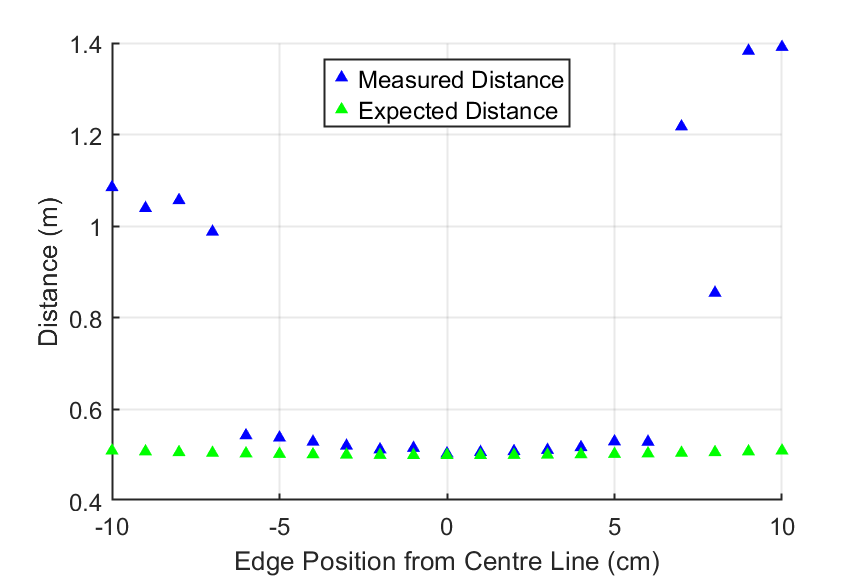
\includegraphics[width=0.8\textwidth]{figs/distAndExpected.png}
    \caption{Average measured distances and expected distances.}
    \label{fig:distandExpected}
\end{figure}

\begin{figure}[htbp]
    \centering
    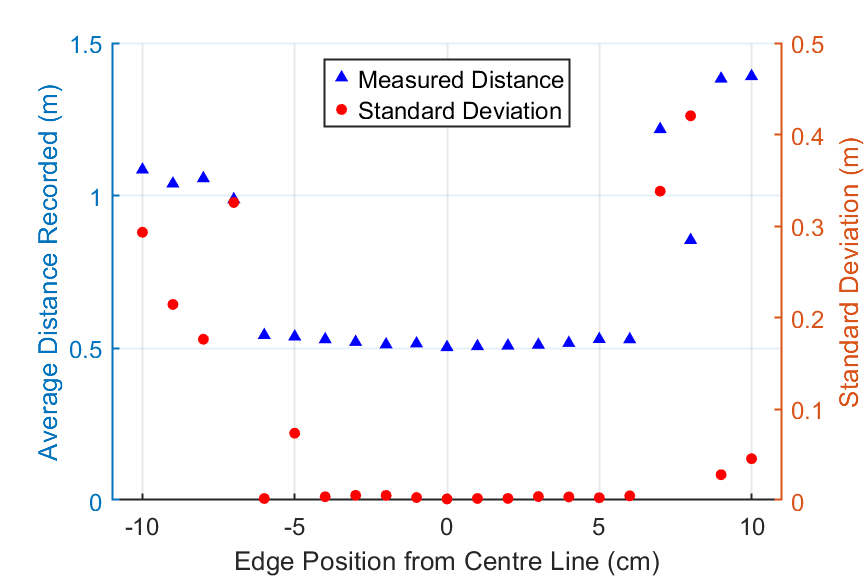
\includegraphics[width=0.8\textwidth]{figs/task2.png}
    \caption{Average measured distances and their standard deviations.}
    \label{fig:distandSE}
\end{figure}

\begin{table}[ht]
    \centering
    \begin{tabular}{lccccccccccc}
        \hline
        $h$ (cm) & 0 & $\pm$1 & $\pm$2 & $\pm$3 & $\pm$4 & $\pm$5 & $\pm$6 & $\pm$7 & $\pm$8 & $\pm$9 & $\pm$10\\
        $\theta$ (°) & 0 & 1.146 & 2.291 & 3.434 & 4.574 & 5.711 & 6.843 & 7.970 & 9.090 & 10.20 & 11.31 \\
        \hline
    \end{tabular}
    \caption{Perpendicular distances at $D_{I}=0.5$m and their corresponding angles.}
    \label{tab:angles}
\end{table}

\break

\subsection{Task 3: Object Detection and Alarm}
The application successfully handled live plotting and outputs, Figure~\ref{fig:task3GUI1}. The save measurement function calls a file explorer window, Figure~\ref{fig:task3GUI2}.
When the rolling average exceeds the calibration range it is displayed in red, Figure~\ref{fig:task3GUI3}
Measurement frequencies of 45Hz could be achieved in certain conditions, Figure~\ref{fig:task3GUI4}.

\begin{figure}[htbp]
    \centering
    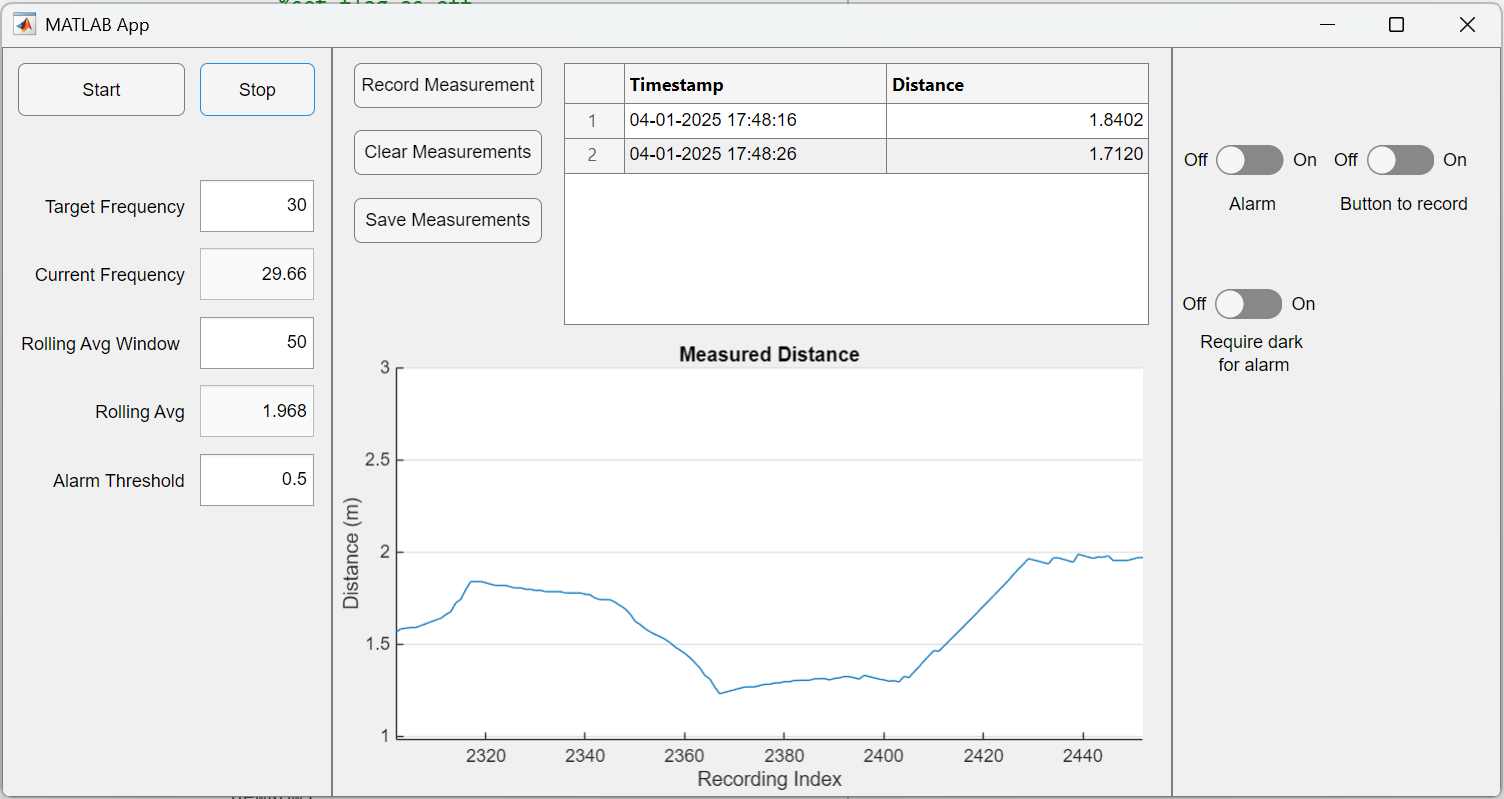
\includegraphics[width=0.8\textwidth]{figs/task3GUI1.png}
    \caption{Screen capture of the GUI showing live plotting and outputs such as current frequency and rolling average.}
    \label{fig:task3GUI1}
\end{figure}


\begin{figure}[htbp]
    \centering
    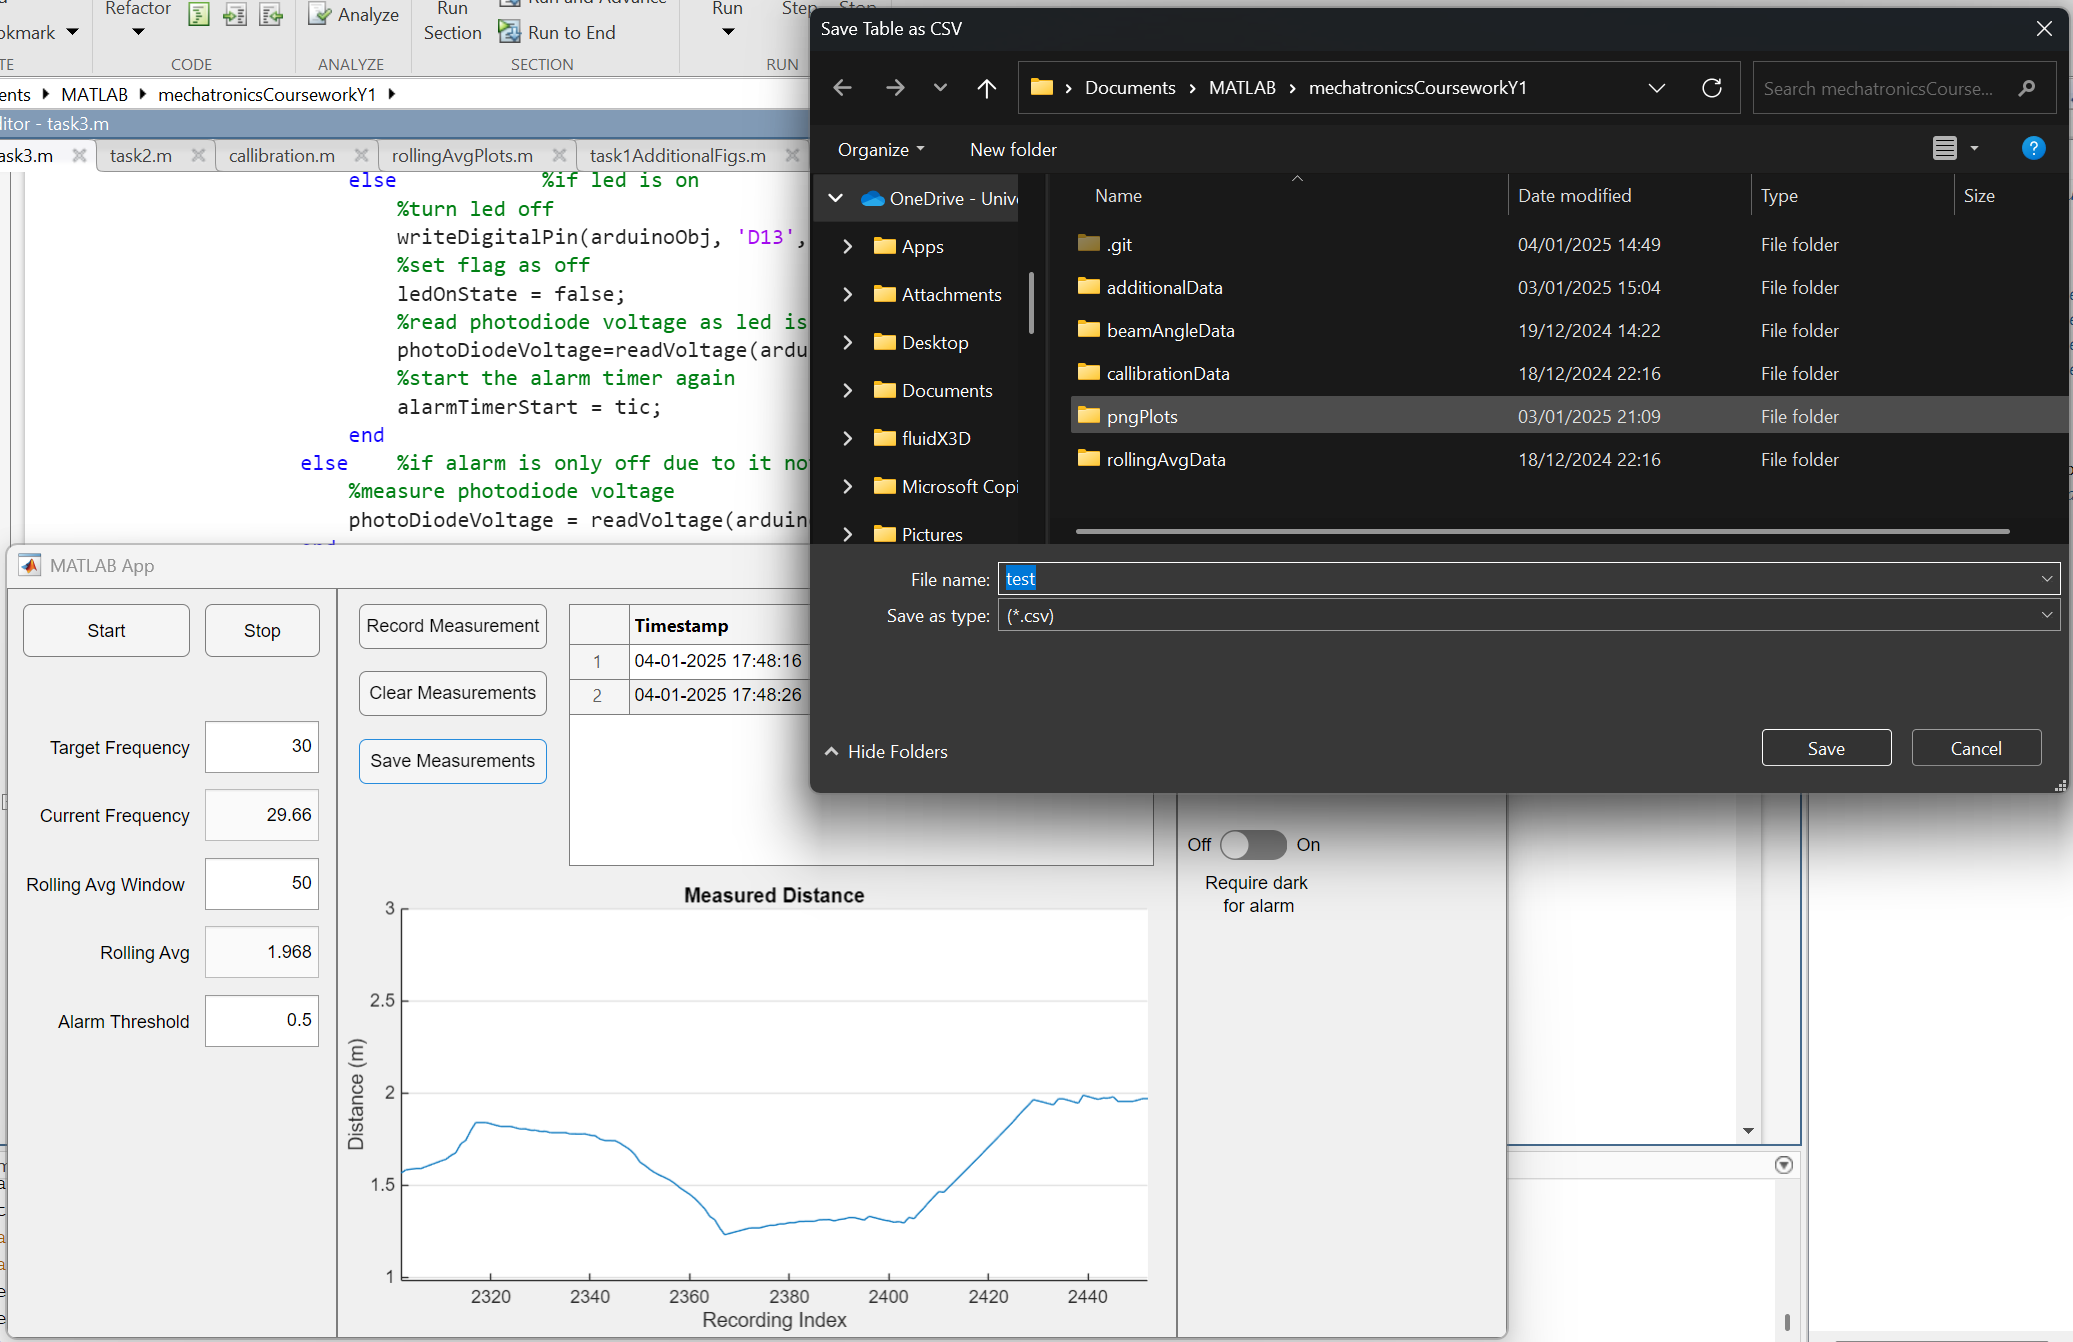
\includegraphics[width=0.8\textwidth]{figs/task3GUI2.png}
    \caption{Screen capture of the GUI showing save recordings functionality and the file explorer window that is opened.}
    \label{fig:task3GUI2}
\end{figure}

\break

The alarm matched it's design requirements, varying the frequency of flashing controlled by the potentiometer and the distance within the alarm threshold. The push-button recording function and the LDR alarm functionality were also tested successfully.

\begin{figure}[htbp]
    \centering
    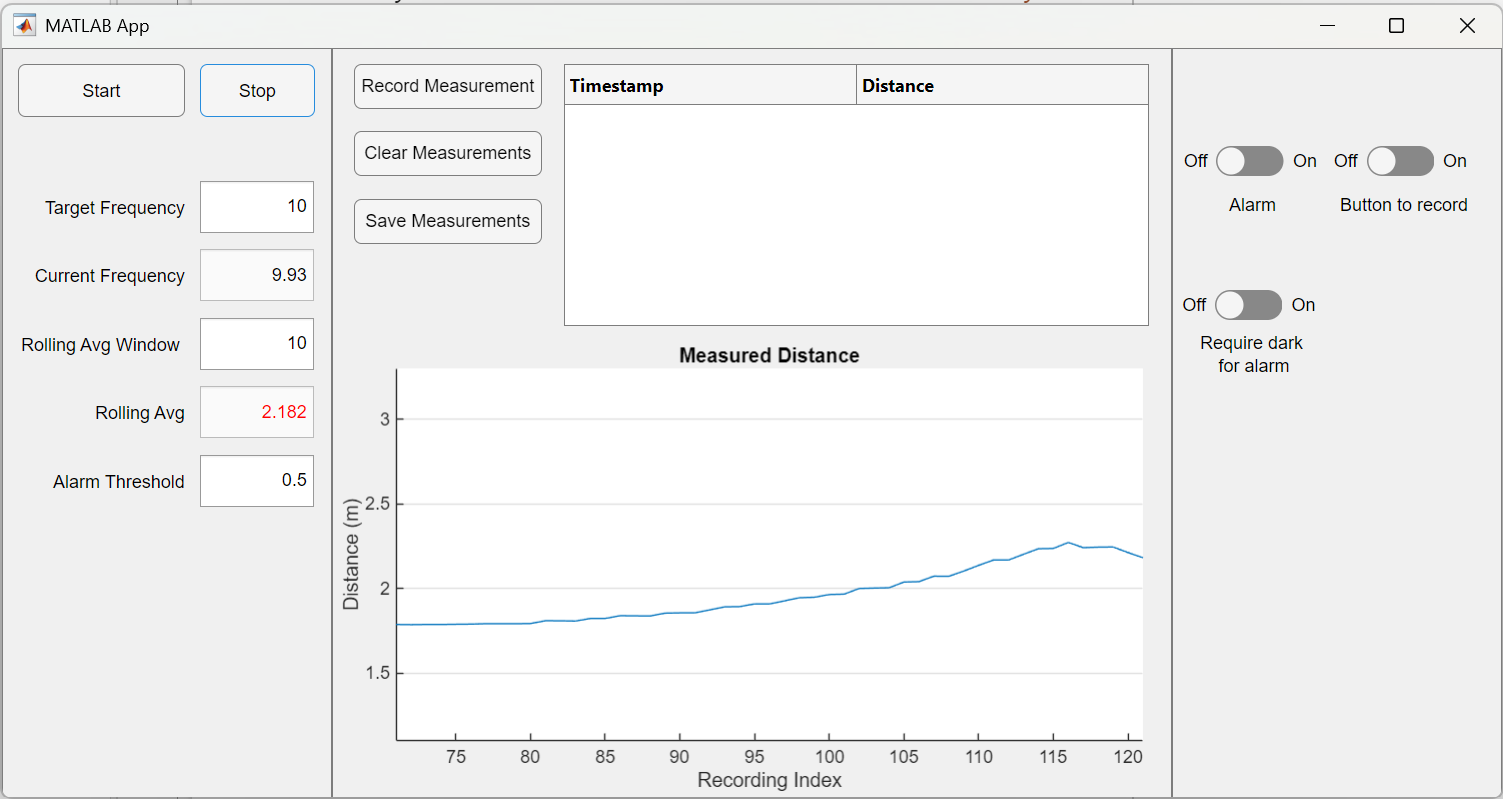
\includegraphics[width=0.8\textwidth]{figs/task3GUI3.png}
    \caption{Screen capture of the GUI showing rolling average displayed in red.}
    \label{fig:task3GUI3}
\end{figure}



\begin{figure}[htbp]
    \centering
    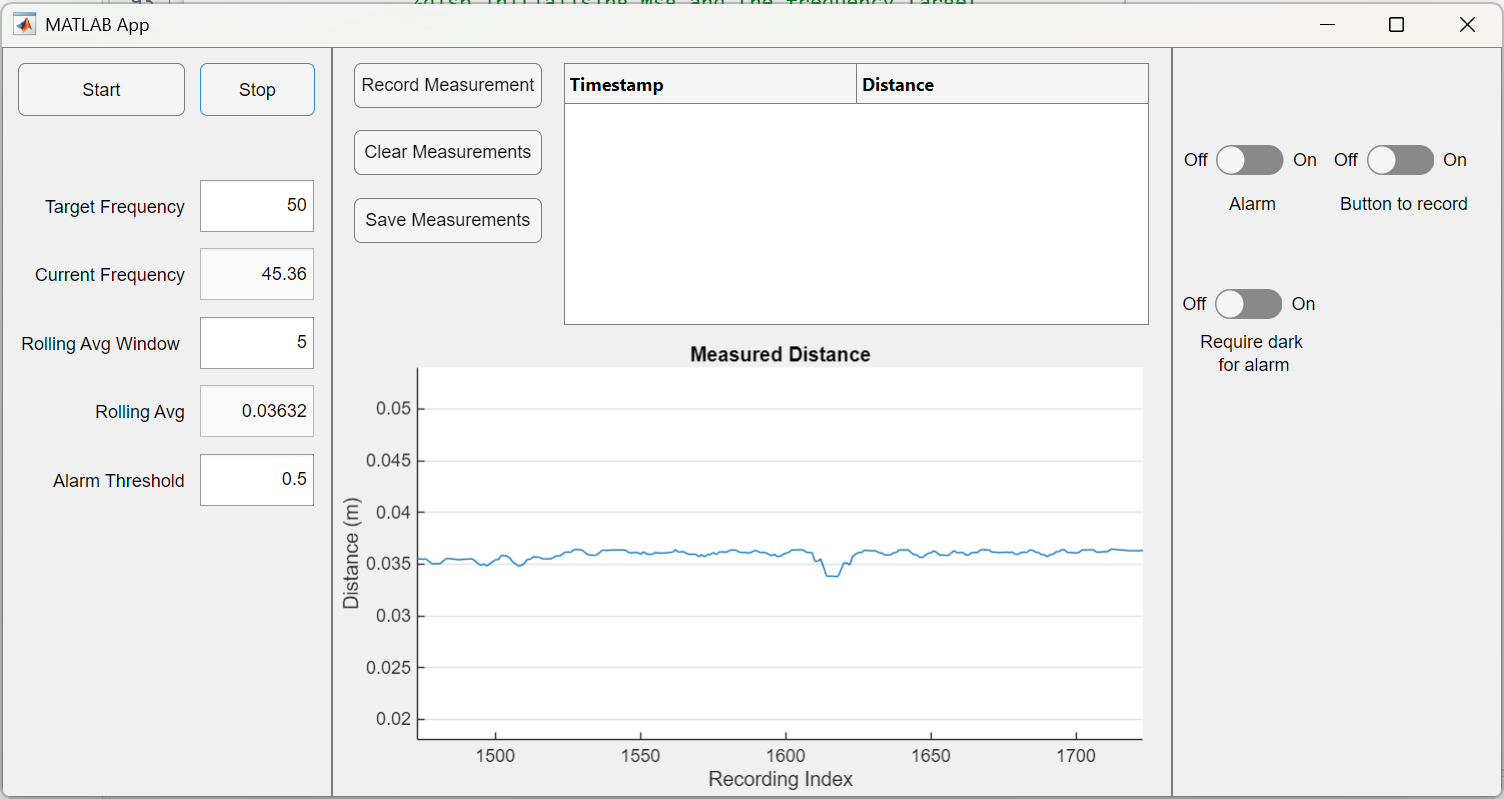
\includegraphics[width=0.8\textwidth]{figs/task3GUI4.png}
    \caption{Screen capture of the GUI showing high measurement frequency.}
    \label{fig:task3GUI4}
\end{figure}


\break


\section{Discussion}

\subsection{Task 1: Sensor Circuit and Arduino Setup}
To select a moving average window, 4 different sizes were evaluated on the same data (Figure~\ref{fig:4windowsize}). There was an increase in smoothness with each larger window, both 25 and 50 point windows had $\sigma$ at or below a 1\% threshold, 25 point was chosen for its shorter time lag. The delay between the smoothed data and raw data can still be seen in Figure~\ref{fig:liveData}. This lag could be reduced by increasing sampling frequency.

Calibration was done from 0.1m to 2.0m, this range was the maximum of the clear test area and covers half the sensor's 4m range (Appendix~\ref{trusens}. The calibration distances were measured to $\pm$1mm. The model's offset of \~1mm and SE of \~2mm (Table~\ref{tab:linearModel}), may be caused by measurement errors in target positioning. Its gradient shows close correlation with the true values and a low uncertainty. The small variation between the model and ideal gradient could be due to variations in the speed of sound, it varies by \~0.2\% per °C \parencite{10.1121/1.391918}. The variation could thusly correspond to an environment temperature 1°C from that of the utilised speed of sound.

The MATLAB script reports measurements outside the calibration range of 0.1m to 2m, but the system should only be used within its calibration range as otherwise the calibration is being extrapolated.
It can be seen in Figure~\ref{fig:liveData} that the system outputs accurate live measurements with a small delay.

\subsection{Task 2: Beam Angle Constraints}

 Average $D_{M}$ exceeds a threshold of 10\% above $D_{E}$ when $|h|>6$cm, Figure~\ref{fig:distandExpected}. This corresponds to an angle of $\pm$6.8°, Table~\ref{tab:angles}. Due to measurement spacing of 1cm (1.15°) the final beam angle is 13.7°$\pm$2.3°. They are close whilst $|h|\leq6$cm but drift as $|h|$ increases. Whilst the beam angle is 13.7°$\pm$2.3°, the accuracy decreases when the target is not in front of the sensor. Another possible cause is the sensor receiver and transmitter are adjacent but independent, the distance between them will influence the TOF as the target angle increases. Another possible cause is reflections from the edge or side face of the target interfering with the pulse.

 Figure~\ref{fig:distandSE} shows $\sigma$ for each measurement, the lowest is at $h=0$, remaining low until $|h|>6$cm except one erroneous measurement at $h=-5$cm. When $|h|>6$cm $\sigma$ is greatly elevated relative to when $|h|\leq6$cm, this indicates that whilst the sensor cannot accurately measure the distance to the target, an echo is still being detected and affecting the measurement. 

Beam angle of the measurement system may be increased without the caveat of reduced range by creating a system fusing aspects of different sensors with different beam angles enabling the functionality of wide and narrow beam sensors as detailed in \cite{4388569}. A change that may prevent the measurement drift as $h$ increases is rotating the sensor to have the receiver and transmitter above each other, or utilise transducer based sensor.

An improvement for general system accuracy could be including a DHT11 temperature and humidity sensor to correct for variations in the speed of sound as implemented by \cite{Berger2023}.

\subsection{Task 3: Object Detection and Alarm}
%The use of a parallel worker allowed for measurement frequencies up to \~45Hz, the maximum frequency readily achieved with task 1 was \~24Hz. However, frequencies were impacted by the measured distance as longer TOF meant less measurements could be taken per second. Other functions such as the alarm limited the maximum frequency, this is due to the slow nature of MATLAB's writeDigitalPin and readVoltage functions. This could be alleviated by implementing custom serial communication. The parallel worker also had other limitations such as difficulty passing in variables once it was started so variables could only be set before measurements were started.
The system could be used effectively for safety within a factory with additional functions like the LDR giving the option that the alarm only functions when it is dark and workers are at risk.
The higher maximum measurement frequencies of \~45Hz compared to the \~24Hz of task 1 are attributed to the use of a parallel worker for measurements and plotting. Frequency was negatively affected by distance as increased TOF means each measurement takes longer. MATLAB's writeDigitalPin and readVoltage functions are slow and limit the frequency to \~10Hz when the alarm is running. This could be alleviated by establishing custom serial communication. Variables/states can only be altered when measurements are not running due to limitations of the parfeval function execution.



\section{Conclusion}
Task 1 improved measurement smoothness from an ultrasonic ranging module by applying moving average filtering, with a window size of 25 selected as a balance between smoothness ($\text{standard deviation}\leq1$mm over a measurement of 1m) and measurement delay. The estimated measurement offset error (-1.35mm$\pm$1.96mm)was low enough to be accounted for by uncertainty in the calibration method. The estimated error factor (0.2\%) was low enough to be accountable to the change of the speed of sound from a 1°C change in environment. 


Task 2 characterised the beam angle constraint as 13.7°$\pm$2.3° for measurements within 10\% of expected values. The low resolution between measurements (1.15°) gives a large uncertainty. An unexpected finding was a drift from expected measurements as the target moves away perpendicularly from in front of the sensor. Measurement drift may be improved using a transducer sensor or by positioning the transmitter above the receiver. Beam angle may be improved by fusing aspects of different sensors and accuracy improved with atmospheric corrections. 


Task 3 created a more complex measurement and alarm system with an improved MATLAB control script featuring a GUI for improved ease of use. Utilising a parallel worker increased the maximum measurement frequencies from 24 Hz in task 1 to 45Hz. The MATLAB Arduino hardware support library was simplified the use of the board but some features were slow, this can be avoided by directly interfacing with the board.


Future work for task 1 may include investigating sensors to calibrate for atmospheric conditions and running measurements in parallel to plotting and other functions. For task 2 it may include investigating the measurement drift and mitigating methods. For task 3 it could include implementing two-way dataQueue communication with the parallel worker for updatable parameters and changes to serial communication.

%TC:ignore

\section{Supplementary Materials}
Scripts, data and plots for this project are available in this Github repository: \url{https://github.com/bigOwlTr/mechatronicsCWY1S1}.

\section{Bibliography}
\newrefcontext[sorting=nyt]
\printbibliography[heading=none]

\appendix
\section{HC-SR504 Data Sheet}
\label{trusens}
Provided in this appendix is the link used to access the data sheet of the utilised HC-SR504 ultrasonic ranging module:
\url{https://static.mercateo.com/3d/a3082259b18446a7a90254737567ea01/pdf/74-1109_v1.pdf}.

\section{MATLAB Code: Task 1}
\label{appendix:A1}
\subsection{Main Measurement Script}
In this appendix is the MATLAB script used for measurements in task 1, it handles measurements at a targeted frequency with a set rolling average. The script also handles rudimentary plotting for visualisation. A debug printout is provided as an option.
\lstinputlisting{code/task1.m}
\subsection{Calibration Script}
\label{appendix:A2}
This appendix contains the MATLAB script used to calculate the measurement errors for calibration along with creating the plots showing the data and linear model.
\lstinputlisting{code/callibration.m}
\subsection{Rolling Average Plots}
This appendix contains the MATLAB script that applies applies four different rolling average window sizes to a dataset, calculates standard deviations and means, then plots the data.
\lstinputlisting{code/rollingAvgPlots.m}
\label{rollingAvgPlots.m}
\subsection{Additional Figures}
This appendix contains the MATLAB script that handles additional plotting for task 1, it plots a dataset with and without the chosen moving average window of 25.
\lstinputlisting{code/task1AdditionalFigs.m}

\section{MATLAB Code: Task 2}
This appendix contains the code used in task 2 that calculates and plots average measured distance, standard deviation and expected distance.
\lstinputlisting{code/task2.m}
\section{MATLAB Code: Task 3}
This appendix contains the code for task 3, a MATLAB app which handles and plots live data along with alarm functionality utilising physical and GUI inputs. The app also utilises parallel execution for greater polling frequencies.
\lstinputlisting{code/task3.m}
\label{Appendix:C}

%TC:endignore

\end{document}
